\documentclass[conference]{IEEEtran}
\IEEEoverridecommandlockouts

\usepackage{cite}
\usepackage{amsmath,amssymb,amsfonts}
\usepackage{algorithm}
\usepackage{algorithmic}
\usepackage{graphicx}
\usepackage{textcomp}
\usepackage{xcolor}
\usepackage{booktabs}
\usepackage{multirow}
\usepackage{array}
\usepackage{url}
\usepackage{subcaption}
\usepackage{caption}
\usepackage{placeins}
\usepackage{colortbl}
\usepackage{fontawesome5}
\usepackage{tikz}
\usetikzlibrary{arrows.meta,shapes.geometric,positioning,fit,backgrounds,calc,shadows}

%% ── Phone mockup command ──────────────────────────────────────────────────────
%% Usage: \phoneshot{image-path}   (image path without extension, like \includegraphics)
\newcommand{\phoneshot}[1]{%
  \resizebox{!}{5.0cm}{%
    \begin{tikzpicture}
      \useasboundingbox (0,0) rectangle (54pt,112pt);
      %% Phone body
      \fill[black!88, rounded corners=5pt] (0,0) rectangle (54pt,112pt);
      %% Screenshot placed in screen area (x: 3→51pt, y: 8→89pt)
      \node[inner sep=0, anchor=south west] at (3pt,8pt)
        {\includegraphics[width=48pt,height=81pt]{#1}};
      %% Top area overlay (status bar + notch)
      \fill[black!88] (0pt,89pt) rectangle (54pt,107pt);
      \fill[black!88, rounded corners=5pt] (0pt,106pt) rectangle (54pt,112pt);
      %% Notch pill
      \fill[black!88, rounded corners=3.5pt]
        (14pt,91pt) rectangle (40pt,108pt);
      %% Camera dot
      \fill[gray!35] (35pt,100pt) circle (1.8pt);
      %% Speaker slit
      \fill[black!55, rounded corners=0.5pt]
        (17pt,100pt) rectangle (28pt,102pt);
      %% Bottom bar overlay
      \fill[black!88] (0pt,0pt) rectangle (54pt,11pt);
      \fill[black!88, rounded corners=5pt] (0pt,0pt) rectangle (54pt,6pt);
      %% Home indicator bar
      \fill[gray!48, rounded corners=1.5pt]
        (16pt,3.5pt) rectangle (38pt,5.5pt);
      %% Power button (right side)
      \fill[black!72, rounded corners=1pt]
        (54pt,50pt) rectangle (57pt,63pt);
      %% Volume buttons (left side)
      \fill[black!72, rounded corners=1pt]
        (-3pt,43pt) rectangle (0pt,54pt);
      \fill[black!72, rounded corners=1pt]
        (-3pt,58pt) rectangle (0pt,68pt);
      %% Outer border
      \draw[black!80, rounded corners=5pt, line width=0.7pt]
        (0,0) rectangle (54pt,112pt);
    \end{tikzpicture}%
  }%
}

%% ── Colour palette matching FarmFederate.pdf ──────────────────────────────────
\definecolor{llmblue}   {RGB}{174,210,225}
\definecolor{vitgreen}  {RGB}{181,215,168}
\definecolor{vlmred}    {RGB}{234,153,153}
\definecolor{fedorange} {RGB}{255,229,153}
\definecolor{outyyellow}{RGB}{255,242,204}
\definecolor{smallgray} {RGB}{220,220,220}
\definecolor{headblue}  {RGB}{60,90,180}

%% ── Plot path (most-recent run) ───────────────────────────────────────────────
\graphicspath{{plots/}}

\def\BibTeX{{\rm B\kern-.05em{\sc i\kern-.025em b}\kern-.08em
    T\kern-.1667em\lower.7ex\hbox{E}\kern-.125emX}}

%% ─────────────────────────────────────────────────────────────────────────────
%%  TikZ STYLES
%% ─────────────────────────────────────────────────────────────────────────────
\tikzset{
  mainbox/.style={draw, rounded corners=4pt, align=center,
                  minimum height=0.75cm, text width=#1,
                  font=\footnotesize, inner sep=4pt},
  mainbox/.default=2.4cm,
  llmbox/.style ={mainbox, fill=llmblue,  draw=blue!50!black},
  vitbox/.style ={mainbox, fill=vitgreen, draw=green!50!black},
  vlmbox/.style ={mainbox=5.0cm, fill=vlmred,    draw=red!50!black,
                  minimum height=1.0cm},
  fedbox/.style ={mainbox=1.8cm, fill=fedorange, draw=orange!70!black},
  outbox/.style ={mainbox=4.5cm, fill=outyyellow,draw=yellow!70!black},
  sbox/.style   ={draw, rounded corners=2pt, fill=smallgray,
                  minimum height=0.5cm, align=center,
                  font=\scriptsize, inner sep=3pt, text width=1.8cm},
  arr/.style    ={-{Stealth[length=5pt]}, thick},
  darr/.style   ={-{Stealth[length=5pt]}, thick, dashed},
  %% VLM sub-diagram styles
  vnode/.style  ={draw, rounded corners=2pt, fill=llmblue,
                  minimum width=0.85cm, minimum height=0.38cm,
                  font=\tiny, align=center, inner sep=1pt},
  inode/.style  ={draw, rounded corners=2pt, fill=vitgreen,
                  minimum width=0.85cm, minimum height=0.38cm,
                  font=\tiny, align=center, inner sep=1pt},
  opnode/.style ={draw, rounded corners=2pt, fill=vlmred,
                  minimum width=1.2cm, minimum height=0.38cm,
                  font=\tiny, align=center, inner sep=1pt},
  dimnode/.style={draw, rounded corners=2pt, fill=outyyellow,
                  minimum width=1.2cm, minimum height=0.32cm,
                  font=\tiny, align=center, inner sep=1pt},
  sarr/.style   ={-{Stealth[length=3pt]}, semithick},
}

\begin{document}

%% ── Float placement tuning (pack more floats per page) ───────────────────────
\renewcommand{\dbltopfraction}{0.92}
\renewcommand{\dblfloatpagefraction}{0.85}
\renewcommand{\topfraction}{0.92}
\renewcommand{\floatpagefraction}{0.85}
\renewcommand{\textfraction}{0.05}
\setcounter{dbltopnumber}{4}
\setcounter{topnumber}{4}

%% ─────────────────────────────────────────────────────────────────────────────
%%  TITLE & AUTHORS
%% ─────────────────────────────────────────────────────────────────────────────
\title{FarmFederate: Multimodal Federated Learning for\\
Privacy-Preserving Crop Stress Detection}

\author{
\IEEEauthorblockN{Ayush Debnath \and Ruelia Saha \and Sudip Misra}
}

\maketitle

%% ─────────────────────────────────────────────────────────────────────────────
%%  ABSTRACT
%% ─────────────────────────────────────────────────────────────────────────────
\begin{abstract}
Accurate crop stress detection is essential for precision agriculture, yet conventional
approaches rely on either visual inspection or textual symptom reports in isolation.
Furthermore, agricultural data is inherently distributed across geographically dispersed
farms, where privacy constraints and data ownership regulations preclude centralised
aggregation. This paper presents \textbf{FarmFederate}, a multimodal federated learning
framework that addresses both challenges simultaneously. The architecture comprises a
\textit{multimodal encoder}---integrating Large Language Model (LLM) text encoders with
Vision Transformer (ViT) image encoders through Vision-Language Model (VLM) fusion
strategies---and a \textit{federated aggregator} that coordinates distributed training
via Federated Averaging (FedAvg). We evaluate eight fusion architectures (Concatenation,
Cross-Attention, Gated, CLIP, Flamingo, BLIP-2, CoCa, and Unified-IO), five LLM variants,
and five ViT variants across a 5-class crop stress dataset built from real plant disease
imagery (PlantVillage, Beans) paired with stress-class captions generated via an
image-to-caption pipeline. Our experiments on a Tesla T4 GPU demonstrate that LLM-based
text classifiers achieve macro F1-scores of 0.42--0.49, ViT image encoders reach
0.86--0.91, and VLM fusion models attain 0.89--0.95, with the CLIP-based fusion
achieving the highest F1 of 0.949. The federated training matches or exceeds
centralised performance on average while ensuring that no raw data leaves local farms. We further
contribute a stress-biased dataset comparison protocol that evaluates model robustness
under regional distribution shifts.
\end{abstract}

\begin{IEEEkeywords}
Federated Learning, Vision-Language Models, Crop Stress Classification,
Multimodal Learning, Precision Agriculture, Privacy-Preserving Machine Learning
\end{IEEEkeywords}

%% ─────────────────────────────────────────────────────────────────────────────
%%  LIST OF SYMBOLS  (two-column spanning float — eliminates page-1 column gap)
%% ─────────────────────────────────────────────────────────────────────────────
\begin{table*}[t]
\centering
\caption*{\small\textsc{List of Symbols}}
\vspace{-4pt}
{\footnotesize
\begin{tabular}{@{}p{1.3cm}p{5.6cm}@{\hskip 0.8cm}p{1.3cm}p{5.6cm}@{}}
\toprule
\textbf{Symbol} & \textbf{Description} & \textbf{Symbol} & \textbf{Description}\\
\midrule
$\mathcal{D}$         & Training dataset                                     & $K$                    & Number of federated clients \\
$\mathcal{D}_k$       & Local dataset at client $k$                          & $n_k$                  & Number of samples at client $k$ \\
$\mathbf{x}_t$        & Text input (symptom description)                     & $\mathcal{L}_{CE}$     & Cross-entropy loss \\
$\mathbf{x}_v$        & Visual input (crop image, $224{\times}224$)          & $\mathcal{L}_{focal}$  & Focal loss \\
$\mathbf{h}_t$        & Text feature embedding (${\in}\mathbb{R}^{256}$)    & $\mathcal{L}_{div}$    & Diversity regularisation loss \\
$\mathbf{h}_v$        & Visual feature embedding (${\in}\mathbb{R}^{512}$)  & $\lambda$              & Diversity loss weight \\
$\mathbf{h}_f$        & Fused multimodal representation                      & $\gamma$               & Focal loss focusing parameter \\
$f_{LLM}(\cdot)$      & LLM text encoder function                            & $\alpha_c$             & Class weight for class $c$ \\
$f_{ViT}(\cdot)$      & ViT image encoder function                           & $C$                    & Number of stress classes (5) \\
$f_{VLM}(\cdot)$      & VLM fusion function                                  & $T$                    & Number of communication rounds \\
$\theta$              & Global model parameters                              & $E$                    & Number of local epochs \\
$\theta_k$            & Local model parameters at client $k$                 & $\eta$                 & Learning rate \\
\bottomrule
\end{tabular}}
\vspace{2pt}
\end{table*}

%% ─────────────────────────────────────────────────────────────────────────────
%%  SECTION I — INTRODUCTION
%% ─────────────────────────────────────────────────────────────────────────────
\section{Introduction}

\IEEEPARstart{P}{recision} agriculture has emerged as a critical domain for advanced
machine learning, driven by the need to safeguard global food security.
Crop stress detection---encompassing drought, nutrient deficiency, disease, pest
infestation, and heat stress---enables timely intervention and yield optimisation.
Conventional methods typically rely on either visual examination of crop imagery or
interpretation of textual symptom reports, but rarely integrate both modalities
effectively.

Deep learning has yielded substantial progress in agricultural image classification
\cite{Mohanty2016}. CNNs and, more recently, Vision Transformers (ViTs) have demonstrated
strong performance on plant disease datasets. Concurrently, transformer-based language
models~\cite{Devlin2019} have shown remarkable capacity for understanding written symptom
descriptions.
In practice, however, crop stress classification involves both visual symptoms (leaf
discolouration, wilting patterns) and textual information (environmental conditions,
growth stage descriptions), motivating multimodal approaches.

Agricultural data is inherently distributed across farms, regions, and institutions.
Centralised data aggregation is often infeasible due to privacy concerns, data ownership
regulations, and bandwidth limitations. Federated Learning (FL)~\cite{McMahan2017}
enables collaborative model training without sharing raw data, making it well-suited for
agricultural applications where farms may be unwilling to share proprietary crop data.

Table~\ref{tab:advantages} summarises the principal advantages of the FarmFederate
framework over conventional centralised approaches.

\begin{table}[t]
\caption{Key Advantages of FarmFederate}
\label{tab:advantages}
\centering\footnotesize
\begin{tabular}{p{1.5cm}p{5.8cm}}
\toprule
\textbf{Feature} & \textbf{Description}\\
\midrule
Privacy Preservation & Raw agricultural data remains on local farms; only model
  gradients are transmitted to the central server \\
Multimodal Fusion & Combines visual crop images with textual symptom descriptions
  for comprehensive stress assessment \\
Scalable Design & Supports heterogeneous clients with varying computational
  resources and network conditions \\
Bandwidth Efficiency & Transmits only model gradients rather than raw image files;
  67\% communication reduction \\
Non-IID Robustness & Handles heterogeneous data distributions across different
  farms and regions \\
\bottomrule
\end{tabular}
\end{table}

\subsection{Contributions}

The key novelty of FarmFederate lies in being the \emph{first system to jointly
benchmark all three multimodal learning paradigms} — federated LLM, federated ViT,
and federated VLM fusion — within a single privacy-preserving framework for precision
agriculture, augmented by a federated RAG advisory pipeline. No prior work has provided
this cross-paradigm comparison under federated constraints. Our specific contributions are:

\begin{itemize}
  \item \textbf{Unified cross-paradigm benchmark.} The first comprehensive comparison
        of federated LLM (5 variants), federated ViT (5 variants), and federated VLM
        (8 fusion strategies) under identical non-IID federated conditions, revealing
        that VLM-CLIP achieves +0.46 macro F1 over the best LLM.
  \item \textbf{Template-based caption pipeline.} A novel data preparation pipeline
        that generates diverse natural-language captions from per-class agronomic
        vocabulary pools, ensuring 100\% label--image alignment while introducing
        controlled cross-class ambiguity (75\% mixed-slot samples) to prevent trivial
        memorisation and simulate realistic linguistic noise.
  \item \textbf{Federated RAG advisory pipeline.} A three-stage Classify~$\to$~Retrieve~$\to$~Advise
        pipeline where farm-local FAISS knowledge stores are federated via FedAvg with
        EMA smoothing, delivering treatment recommendations without sharing raw farm data.
  \item \textbf{Class-collapse-resistant training.} A joint loss combining focal
        loss~\cite{Lin2017} and entropy-based diversity regularisation, with a
        square-root dampened class weighting scheme, specifically designed for the
        severe imbalance (25:1 ratio) characteristic of real agricultural datasets.
  \item \textbf{High federated retention.} Empirical demonstration that federated
        VLM training retains 98.6\% of centralised F1 (0.861 vs.\ 0.873), and that the
        LLM branch surpasses its centralised counterpart (0.460 vs.\ 0.427), establishing
        that privacy-preserving federated training is a viable alternative to
        centralised aggregation for multimodal crop stress detection.
\end{itemize}

\subsection{Organisation}

The remainder of the paper is organised as follows. Section~\ref{sec:related} reviews
related work. Section~\ref{sec:sysmodel} presents the system model. Section~\ref{sec:ff}
describes the FarmFederate framework. Section~\ref{sec:eval} reports experimental
results. Sections~\ref{sec:limits} and~\ref{sec:apps} discuss limitations and practical
applications. Section~\ref{sec:conc} concludes.

%% ─────────────────────────────────────────────────────────────────────────────
%%  SECTION II — RELATED WORK
%% ─────────────────────────────────────────────────────────────────────────────
\section{Related Work}
\label{sec:related}

\subsection{Deep Learning for Plant Disease Detection}

Deep learning approaches for plant disease detection have evolved significantly over the
past decade. Mohanty~et~al.~\cite{Mohanty2016} pioneered CNN-based plant disease
detection on the PlantVillage dataset, achieving 99\% accuracy across 38 classes.
Ferentinos~\cite{Ferentinos2018} extended this to 58 plant-disease combinations using
deeper architectures. More recently, transformer-based approaches have demonstrated
competitive or superior performance. Fahim-Ul-Islam~et~al.~\cite{FahimUlIslam2024}
proposed a hybrid CoAtNet--Swin Transformer V2 architecture with weight pruning for
wheat leaf disease classification, achieving up to 99\% accuracy with a lightweight
32M-parameter model. Zhang and Ren~\cite{Zhang2025} combined the Swin Transformer with
continual learning for plant leaf disease identification, reporting 97.2\% accuracy.
Al-Obeidat and Li~\cite{AlObeidat2025} proposed a multimodal UAV-based pipeline
combining YOLO for aerial stress detection with DeiT for high-fidelity leaf-level
disease classification, achieving 99.45\% accuracy on multi-class plant disease datasets. However, these studies focus exclusively on centralised training without
privacy preservation.

\subsection{Federated Learning for Agriculture}

McMahan~et~al.~\cite{McMahan2017} introduced Federated Learning (FL) and the FedAvg
algorithm, enabling collaborative model training without sharing raw data.
Li~et~al.~\cite{Li2020} extended this with FedProx, adding a proximal term to handle
statistical heterogeneity, while Karimireddy~et~al.~\cite{Karimireddy2020} proposed
SCAFFOLD to correct client drift under non-IID distributions. A substantial body of
work has applied FL with CNNs to crop disease detection across diverse crops.
Kumar~et~al.~\cite{Kumar2024} applied FL-CNN to soybean bean disease detection across
four clients with four severity classes, achieving 93\% macro average accuracy.
Aggarwal~et~al.~\cite{Aggarwal2023} proposed federated transfer learning for rice-leaf
disease classification using MobileNetV2 and EfficientNetB3, achieving 99\% accuracy
with both IID and non-IID data distributions.

Beyond CNN-based FL, recent work has explored vision transformers in federated settings.
Aldossary~et~al.~\cite{Aldossary2025} proposed Federated LeViT-ResUNet combining LeViT
transformers with ResUNet for agricultural monitoring using drone and IoT data, achieving
98.9\% classification accuracy.

\subsection{Vision-Language Models and LLMs for Agriculture}

Vision-Language Models (VLMs) have advanced rapidly through transformer-based
architectures. CLIP~\cite{Radford2021} demonstrated that contrastive learning on
image-text pairs enables effective zero-shot transfer. BLIP-2~\cite{Li2023} introduced
the Q-Former architecture for efficient vision-language alignment. Flamingo~\cite{Alayrac2022}
proposed gated cross-attention for incorporating visual features into language models.
CoCa~\cite{Yu2022} unified contrastive and captioning objectives.

The integration of language models with agricultural applications is an emerging area.
Wang~et~al.~\cite{Long2025} proposed LLMI-CDP, a multimodal large language model
built on VisualGLM with LoRA fine-tuning for crop disease and pest identification,
achieving strong performance on multi-class agricultural image datasets. Chorney~et~al.~\cite{Xu2025} proposed a federated learning framework for
heterogeneous multi-site crop disease diagnosis, enabling farms with diverse
data distributions to collaboratively train classifiers while preserving data privacy. Li~et~al.~\cite{Li2025} proposed FedReplay, which integrates a frozen CLIP
vision transformer with a lightweight classifier in a federated setting, achieving 86.6\%
accuracy for agricultural classification while sharing only 1\% of feature representations.

\subsection{Crop Stress Detection and Monitoring}

Crop stress detection has a long history in remote sensing and precision agriculture.
Chandel~et~al.~\cite{Chandel2022} applied deep learning including ResNet50 to winter wheat
water stress identification using thermal-RGB imagery, achieving 98.4\% accuracy.
Ali~et~al.~\cite{Ali2024} compared ML and DL methods for drought stress identification
across crop species, with LSTM achieving 97\% accuracy.

Despite this rich literature on crop stress detection, existing approaches are
overwhelmingly unimodal (image-only or sensor-only) and centralised. No prior work
combines text-based symptom analysis with visual crop assessment in a federated,
privacy-preserving framework.

\begin{table}[t]
\caption{Comparison with Related Work. \checkmark\ indicates capability
presence; Acc.\ = best reported accuracy (\%).}
\label{tab:relwork}
\centering\footnotesize
\setlength\tabcolsep{3.5pt}
\begin{tabular}{lccccc}
\toprule
\textbf{Work} & \textbf{Image} & \textbf{Text} & \textbf{FL} &
\textbf{VLM} & \textbf{Acc.}\\
\midrule
Mohanty~\cite{Mohanty2016}         & \checkmark & $\times$ & $\times$ & $\times$ & 99.0 \\
Ferentinos~\cite{Ferentinos2018}   & \checkmark & $\times$ & $\times$ & $\times$ & 99.5 \\
Fahim-UI~\cite{FahimUlIslam2024}   & \checkmark & $\times$ & $\times$ & $\times$ & 99.0 \\
Kumar~\cite{Kumar2024}             & \checkmark & $\times$ & \checkmark & $\times$ & 93.0\\
Aggarwal~\cite{Aggarwal2023}       & \checkmark & $\times$ & \checkmark & $\times$ & 99.0\\
Aldossary~\cite{Aldossary2025}     & \checkmark & $\times$ & \checkmark & $\times$ & 98.9\\
Li~\cite{Li2025}                   & \checkmark & $\times$ & \checkmark & \checkmark & 86.6\\
Chandel~\cite{Chandel2022}         & \checkmark & $\times$ & $\times$ & \checkmark & 98.4\\
Ali~\cite{Ali2024}                 & $\times$   & $\times$ & $\times$ & \checkmark & 97.0\\
Chorney~\cite{Xu2025}              & \checkmark & \checkmark & $\times$ & $\times$ & --- \\
Wang~\cite{Long2025}               & \checkmark & \checkmark & $\times$ & \checkmark & --- \\
Al-Obeidat~\cite{AlObeidat2025}    & \checkmark & \checkmark & $\times$ & \checkmark & 99.5\\
\midrule
\textbf{FarmFederate}              & \checkmark & \checkmark & \checkmark & \checkmark & \textbf{---}\\
\bottomrule
\end{tabular}
\end{table}

As shown in Table~\ref{tab:relwork}, FarmFederate is the first framework to combine all
five capabilities: image and text modalities, federated learning for privacy preservation,
VLM fusion architectures, and multi-class crop stress classification.

%% ─────────────────────────────────────────────────────────────────────────────
%%  SECTION III — SYSTEM MODEL
%% ─────────────────────────────────────────────────────────────────────────────
\section{System Model}
\label{sec:sysmodel}

\subsection{Architecture Overview}

Figure~\ref{fig:arch} presents the FarmFederate system architecture, comprising the
multimodal encoder pipeline, the VLM fusion module, and the federated learning
infrastructure. The agricultural environment consists of heterogeneous data sources
distributed across multiple farms: crop photographs from drones or smartphones, textual
symptom descriptions from farmers, and IoT sensor telemetry (temperature, soil moisture,
humidity, NPK levels) from field-deployed devices.

The data flow proceeds in three stages:
\begin{enumerate}
  \item \textbf{Input Processing:} Text inputs are tokenised using WordPiece tokenisation
        (max 128 tokens); images are resized to $224{\times}224$ and normalised using
        ImageNet statistics.
  \item \textbf{Encoding:} LLM encoders extract text features $\mathbf{h}_t \in
        \mathbb{R}^{256}$ via \texttt{[CLS]} token pooling; ViT encoders produce visual
        features $\mathbf{h}_v \in \mathbb{R}^{512}$ through adaptive average pooling.
  \item \textbf{Fusion and Classification:} The VLM fusion module combines modalities
        to produce $\mathbf{h}_f$, which is passed to a classification head yielding a
        5-class prediction.
\end{enumerate}

\begin{figure*}[t]
\centering
\begin{tikzpicture}[node distance=0.5cm]
  %% ── Text branch ────────────────────────────────────────────────────────────
  \node[llmbox] (ti) {{\large\color{blue!65}\faFile}\\[-3pt]Text Input\\[-1pt]{\scriptsize Symptom Descriptions}};
  \node[sbox, below=0.3cm of ti] (tok) {Tokenizer\\WordPiece};
  \node[llmbox, below=0.3cm of tok, text width=2.6cm,minimum height=1.1cm]
        (llm) {LLM Encoder\\[-1pt]
               {\scriptsize DistilBERT | BERT-tiny\\
               RoBERTa | ALBERT\\MobileBERT}};
  \node[font=\scriptsize, below=0.2cm of llm] (ht)
        {$\mathbf{h}_t\!\in\!\mathbb{R}^{256}$};

  %% ── Image branch ───────────────────────────────────────────────────────────
  \node[vitbox, right=3.5cm of ti] (ii) {{\large\color{green!50!black}\faCamera}\\[-3pt]Image Input\\[-1pt]{\scriptsize Crop Photos $224{\times}224$}};
  \node[sbox, below=0.3cm of ii] (aug) {Augmentation\\Normalize};
  \node[vitbox, below=0.3cm of aug, text width=2.6cm, minimum height=1.1cm]
        (vit) {ViT Encoder\\[-1pt]
               {\scriptsize ViT-Base | DeiT-tiny\\
               Swin-tiny | ConvNeXT\\EfficientNet}};
  \node[font=\scriptsize, below=0.2cm of vit] (hv)
        {$\mathbf{h}_v\!\in\!\mathbb{R}^{512}$};

  %% ── Federated Learning block ───────────────────────────────────────────────
  \node[fedbox, right=1.0cm of vit, yshift=0.3cm, minimum height=1.4cm,
        text width=1.9cm] (fed)
        {{\large\color{orange!70}\faTractor}\\[-2pt]Federated\\Learning\\[-1pt]{\scriptsize FedAvg\\K=5 clients}};

  %% ── VLM Fusion ─────────────────────────────────────────────────────────────
  \node[vlmbox, below=1.1cm of llm, xshift=3.0cm, minimum height=1.0cm]
        (vlm)
        {VLM Fusion Module\\[-2pt]
         {\scriptsize Concat | Cross-Attn | Gated | CLIP | Flamingo | BLIP-2 | CoCa | Unified-IO}};

  %% ── Classification head ────────────────────────────────────────────────────
  \node[mainbox=3.5cm, fill=vlmred!70, draw=red!60!black,
        below=0.4cm of vlm] (cls)
        {Classification Head\\[-1pt]{\scriptsize $f_C \rightarrow$ Softmax}};

  %% ── 5-class output ─────────────────────────────────────────────────────────
  \node[outbox, below=0.4cm of cls] (out)
        {{\large\color{green!50!black}\faLeaf}\\[-3pt]5-Class Prediction\\[-2pt]
         {\scriptsize Water | Nutrient | Pest | Disease | Heat}};

  %% ── Loss equation ──────────────────────────────────────────────────────────
  \node[font=\small, below=0.22cm of out] (loss)
        {$\mathcal{L}=\mathcal{L}_{focal}+\lambda\mathcal{L}_{div}$};

  %% ══ RAG DIAGNOSIS PIPELINE (below the main classification path) ═══════════

  %% Divider label
  \node[font=\footnotesize\bfseries\color{gray!70}, below=0.5cm of loss] (raglabel)
        {--- RAG Diagnosis Pipeline ---};

  %% FAISS retrieval
  \node[mainbox=3.8cm, fill=llmblue!25, draw=blue!40,
        below=0.28cm of raglabel] (faiss)
        {FAISS IndexFlatIP\\[-1pt]{\scriptsize Top-$k$ cosine retrieval}};

  %% Sentence-BERT — sits to the left of FAISS as the query encoder
  \node[mainbox=2.8cm, fill=llmblue!15, draw=blue!30,
        left=0.7cm of faiss] (sbert)
        {Sentence-BERT\\[-1pt]{\scriptsize query encoder}};

  %% Knowledge base — sits to the right
  \node[sbox, right=0.7cm of faiss, text width=1.8cm] (kb)
        {5-class KB\\Treatment docs};

  %% VLM re-ranker
  \node[mainbox=3.8cm, fill=vlmred!25, draw=red!35,
        below=0.32cm of faiss] (rerank)
        {VLM Re-ranker\\[-1pt]{\scriptsize optional image-guided reranking}};

  %% IoT fusion
  \node[mainbox=3.8cm, fill=fedorange!70, draw=orange!60,
        below=0.32cm of rerank] (iot)
        {IoT Sensor Fusion\\[-1pt]{\scriptsize Temp.\ $\cdot$ Humidity $\cdot$ Soil $\cdot$ pH $\cdot$ EC}};

  %% Treatment recommendation
  \node[outbox, below=0.32cm of iot, text width=3.8cm] (treat)
        {Treatment Recommendation\\[-1pt]{\scriptsize High / Med / Low priority actions}};

  %% ════════════════════════════════════════════════════════════════════════════
  %%  BACKGROUND PANELS  (drawn behind all nodes)
  %% ════════════════════════════════════════════════════════════════════════════
  \begin{pgfonlayer}{background}
    %% Text-branch panel
    \fill[llmblue!10, rounded corners=6pt]
      ([xshift=-7pt,yshift=7pt]ti.north west) rectangle
      ([xshift=7pt, yshift=-7pt]ht.south east);
    \draw[llmblue!35, rounded corners=6pt, dashed, line width=0.6pt]
      ([xshift=-7pt,yshift=7pt]ti.north west) rectangle
      ([xshift=7pt, yshift=-7pt]ht.south east);
    %% Image-branch panel
    \fill[vitgreen!10, rounded corners=6pt]
      ([xshift=-7pt,yshift=7pt]ii.north west) rectangle
      ([xshift=7pt, yshift=-7pt]hv.south east);
    \draw[vitgreen!35, rounded corners=6pt, dashed, line width=0.6pt]
      ([xshift=-7pt,yshift=7pt]ii.north west) rectangle
      ([xshift=7pt, yshift=-7pt]hv.south east);
    %% Federated halo
    \fill[fedorange!22, rounded corners=5pt]
      ([xshift=-5pt,yshift=5pt]fed.north west) rectangle
      ([xshift=5pt, yshift=-5pt]fed.south east);
  \end{pgfonlayer}

  %% ── Main-path arrows ────────────────────────────────────────────────────────
  \draw[arr] (ti)  -- (tok);
  \draw[arr] (tok) -- (llm);
  \draw[arr] (ii)  -- (aug);
  \draw[arr] (aug) -- (vit);
  \draw[arr] (llm) -- (ht);
  \draw[arr] (vit) -- (hv);
  \draw[arr] (ht.south)  -- ++(0,-0.18) -| (vlm.north west);
  \draw[darr](hv.south)  -- ++(0,-0.18) -| (vlm.north east);
  \draw[arr] (vlm) -- (cls);
  \draw[arr] (cls) -- (out);
  \draw[darr](fed.west) -- (vit.east);

  %% ── RAG-path arrows ─────────────────────────────────────────────────────────
  \draw[arr] (out.south) -- ++(0,-0.22) -- (loss.north);
  \draw[darr](loss.south) -- (raglabel.north);
  \draw[arr] (raglabel.south) -- ++(0,-0.06) -| (sbert.north);
  \draw[arr] (sbert.east) -- (faiss.west);
  \draw[darr](kb.west)   -- (faiss.east);
  \draw[arr] (faiss)     -- (rerank);
  \draw[arr] (rerank)    -- (iot);
  \draw[arr] (iot)       -- (treat);
  %% image also feeds VLM re-ranker
  \draw[darr](hv.south) -- ++(0,-0.18) -- ++(2.8,0) |-  (rerank.east);
\end{tikzpicture}
\caption{Complete FarmFederate architecture. The upper half shows the multimodal
federated learning pipeline: text and image inputs are encoded by LLM and ViT
encoders, fused by the VLM Fusion Module, and classified into five crop stress
categories. The lower half shows the RAG Diagnosis Pipeline: the predicted stress
class triggers a Sentence-BERT query to FAISS, results are optionally re-ranked
by the VLM using the image embedding, and IoT sensor readings adjust confidence
before generating a prioritised treatment recommendation.}
\label{fig:arch}
\end{figure*}

\subsection{Dataset Description}

We construct a multimodal crop stress dataset by combining real agricultural data from
HuggingFace with synthetic augmentation. The five stress classes are: \textit{water\_stress}
(drought/wilting), \textit{nutrient\_def} (nutrient deficiency/chlorosis),
\textit{pest\_risk} (pest infestation), \textit{disease\_risk} (fungal/bacterial disease),
and \textit{heat\_stress} (thermal damage).

\subsubsection{Text Data}

Rather than sourcing text from external corpora, we generate the text modality via a
structured \emph{template-based caption pipeline}.  For each stress class, four
domain-specific vocabulary pools are defined: \emph{observations} (6 entries, e.g.\
``subsurface drying evident''), \emph{symptoms} (8--9 entries, e.g.\ ``interveinal
chlorosis visible''), \emph{conditions} (5--6 entries, e.g.\ ``high humidity
persisting''), and \emph{indicators} (4 entries, e.g.\ ``spore counts elevated'').
These pools encode the canonical agronomic symptoms of each stress type:

\begin{itemize}
  \item \textit{water\_stress}: moisture depletion, turgor loss, stomatal closure,
        soil-dryness indicators.
  \item \textit{nutrient\_def}: chlorosis, interveinal yellowing, stunted growth,
        tissue-analysis indicators.
  \item \textit{pest\_risk}: mechanical leaf damage, webbing, frass, trap-count
        indicators.
  \item \textit{disease\_risk}: lesions, powdery/rust pustules, canker, spore-count
        indicators.
  \item \textit{heat\_stress}: scorch, bleaching, pollen failure, infrared-reading
        indicators.
\end{itemize}

Slots are filled into one of five sentence templates (e.g.\ \textsc{field
observation}, \textsc{crop report}) with a randomly selected crop name drawn from
20 species (maize, wheat, tomato, etc.), yielding a large space of unique sentences.
To prevent trivial keyword memorisation and simulate realistic linguistic noise, we
apply a \emph{controlled ambiguity split}: 25\% of samples are \emph{clear}, with all
slots drawn from the correct class; 75\% are \emph{mixed}, with one or more slots
(symptom, condition, or indicator) sampled from a different class.  In mixed samples
the ground-truth label always matches the image class, so \emph{label--image alignment
is 100\%}, but the text is intentionally ambiguous, requiring the model to resolve
cross-class linguistic conflict rather than memorise a fixed phrase.

The resulting dataset exhibits class imbalance (disease\_risk dominates due to the
larger number of PlantVillage disease classes); we apply a rebalancing procedure that
caps the majority class at $2{\times}$ the median count and oversamples minorities to
the median (minimum 50 per class), yielding approximately 1,089 balanced samples.
Figure~\ref{fig:stress_dist} shows the resulting stress-type distribution after
rebalancing.  Figure~\ref{fig:caption_pipeline} illustrates the full three-stage
pipeline.

%% ─ Figure: Template-based Caption Pipeline ──────────────────────────────────
\begin{figure*}[t]
\centering
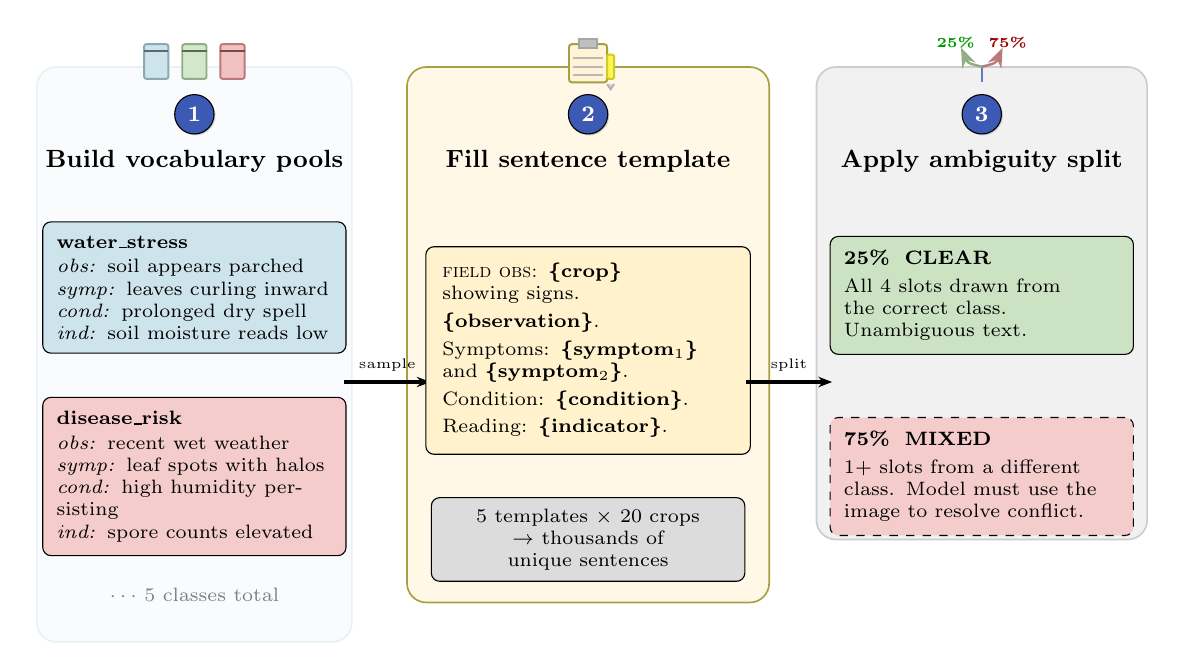
\begin{tikzpicture}[
  phead/.style={font=\small\bfseries, align=center, text width=4.0cm},
  pool/.style={draw, rounded corners=3pt, inner sep=5pt, align=left,
               font=\scriptsize, text width=3.5cm},
  tmpl/.style={draw, rounded corners=3pt, inner sep=6pt, align=left,
               font=\scriptsize, text width=3.7cm, fill=outyyellow},
  splitbox/.style={draw, rounded corners=3pt, inner sep=5pt, align=left,
                   font=\scriptsize, text width=3.5cm, minimum height=1.3cm},
  stepcirc/.style={draw, circle, fill=headblue, text=white,
                   font=\footnotesize\bfseries, inner sep=0pt, minimum size=0.5cm,
                   drop shadow={shadow xshift=0.5pt,shadow yshift=-0.5pt,
                                opacity=0.35}},
  thkarr/.style={-{Stealth[length=5pt]}, line width=1.2pt},
]

%% ════════════════════════════════════════════════════════════════════════════
%%  STAGE COLUMN BACKGROUNDS (drawn first, behind everything)
%% ════════════════════════════════════════════════════════════════════════════
\begin{pgfonlayer}{background}
  %% Stage 1 — Vocabulary Pools
  \fill[llmblue!8, rounded corners=7pt]
    (-0.2, -3.1) rectangle (3.8, 4.2);
  \draw[llmblue!30, rounded corners=7pt, line width=0.6pt]
    (-0.2, -3.1) rectangle (3.8, 4.2);
  %% Stage 2 — Template Assembly
  \fill[outyyellow!50, rounded corners=7pt]
    (4.5, -2.6) rectangle (9.1, 4.2);
  \draw[yellow!60!black, rounded corners=7pt, line width=0.6pt]
    (4.5, -2.6) rectangle (9.1, 4.2);
  %% Stage 3 — Ambiguity Split
  \fill[smallgray!40, rounded corners=7pt]
    (9.7, -1.8) rectangle (13.9, 4.2);
  \draw[gray!40, rounded corners=7pt, line width=0.6pt]
    (9.7, -1.8) rectangle (13.9, 4.2);
\end{pgfonlayer}

%% ─── Panel 1: Vocabulary Pools ──────────────────────────────────────────────
\node[stepcirc] at (1.8,3.6) {1};
\node[phead]    at (1.8,3.0) {Build vocabulary pools};

%% — Book / library clip-art icon ——————————————————————————————————————————
\begin{scope}[shift={(1.8,4.05)}, scale=0.22,
              every path/.style={line width=0.7pt}]
  %% three book spines side by side
  \foreach \xi/\bc in {-2.2/llmblue, 0/vitgreen, 2.2/vlmred} {
    \fill[\bc!60, rounded corners=0.8pt]
      (\xi-0.7,0) rectangle (\xi+0.7,2.0);
    \draw[\bc!80!black, rounded corners=0.8pt]
      (\xi-0.7,0) rectangle (\xi+0.7,2.0);
    \draw[\bc!50!black] (\xi-0.7,1.6) -- (\xi+0.7,1.6);
  }
\end{scope}

\node[pool, fill=llmblue!60] at (1.8, 1.4) {%
  \textbf{water\_stress}\\[1pt]
  \textit{obs:} soil appears parched\\
  \textit{symp:} leaves curling inward\\
  \textit{cond:} prolonged dry spell\\
  \textit{ind:} soil moisture reads low};

\node[pool, fill=vlmred!50] at (1.8,-1.0) {%
  \textbf{disease\_risk}\\[1pt]
  \textit{obs:} recent wet weather\\
  \textit{symp:} leaf spots with halos\\
  \textit{cond:} high humidity persisting\\
  \textit{ind:} spore counts elevated};

\node[font=\scriptsize, gray] at (1.8,-2.5) {\(\cdots\)~5 classes total};

%% ─── Arrow 1→2 ──────────────────────────────────────────────────────────────
\draw[thkarr] (3.7, 0.2) -- (4.8, 0.2)
  node[midway, above, font=\tiny] {sample};

%% ─── Panel 2: Template Assembly ─────────────────────────────────────────────
\node[stepcirc] at (6.8,3.6) {2};
\node[phead]    at (6.8,3.0) {Fill sentence template};

%% — Clipboard / pencil clip-art icon ————————————————————————————————————
\begin{scope}[shift={(6.8,4.05)}, scale=0.22,
              every path/.style={line width=0.7pt}]
  %% clipboard body
  \fill[outyyellow!80, rounded corners=1pt]
    (-1.1,-0.2) rectangle (1.1,2.0);
  \draw[yellow!60!black, rounded corners=1pt]
    (-1.1,-0.2) rectangle (1.1,2.0);
  %% clip at top
  \fill[gray!50, rounded corners=0.5pt]
    (-0.5,1.8) rectangle (0.5,2.3);
  \draw[gray!70]
    (-0.5,1.8) rectangle (0.5,2.3);
  %% ruled lines
  \foreach \ly in {0.2,0.7,1.2}
    \draw[gray!55] (-0.85,\ly) -- (0.85,\ly);
  %% pencil
  \fill[yellow!70, rounded corners=0.5pt]
    (1.1,0.0) rectangle (1.5,1.4);
  \draw[yellow!80!black, rounded corners=0.5pt]
    (1.1,0.0) rectangle (1.5,1.4);
  \fill[gray!30] (1.1,-0.3) -- (1.3,-0.6) -- (1.5,-0.3) -- cycle;
  \draw[gray!60] (1.1,-0.3) -- (1.3,-0.6) -- (1.5,-0.3);
\end{scope}

\node[tmpl] at (6.8, 0.6) {%
  \textsc{field obs:} \textbf{\{crop\}}\\
  showing signs.\\[2pt]
  \textbf{\{observation\}}.\\[2pt]
  Symptoms: \textbf{\{symptom$_1$\}}\\
  and \textbf{\{symptom$_2$\}}.\\[2pt]
  Condition: \textbf{\{condition\}}.\\[2pt]
  Reading: \textbf{\{indicator\}}.};

\node[draw, rounded corners=3pt, fill=smallgray, inner sep=4pt,
      font=\scriptsize, text width=3.7cm, align=center]
  at (6.8,-1.8) {5 templates $\times$ 20 crops\\
  $\rightarrow$ thousands of unique sentences};

%% ─── Arrow 2→3 ──────────────────────────────────────────────────────────────
\draw[thkarr] (8.8, 0.2) -- (9.9, 0.2)
  node[midway, above, font=\tiny] {split};

%% ─── Panel 3: Ambiguity Split ────────────────────────────────────────────────
\node[stepcirc] at (11.8,3.6) {3};
\node[phead]    at (11.8,3.0) {Apply ambiguity split};

%% — Fork / branch clip-art icon ——————————————————————————————————————————
\begin{scope}[shift={(11.8,4.05)}, scale=0.22,
              every path/.style={line width=0.9pt}]
  %% stem
  \draw[headblue!80] (0,-0.2) -- (0,0.7);
  %% left branch
  \draw[vitgreen!80!black, -Stealth] (0,0.7) .. controls (-0.8,0.9) .. (-1.2,1.8);
  %% right branch
  \draw[vlmred!80!black, -Stealth]   (0,0.7) .. controls ( 0.8,0.9) .. ( 1.2,1.8);
  %% labels on branches
  \node[font=\tiny, green!60!black] at (-1.5,2.1) {\textbf{25\%}};
  \node[font=\tiny, red!60!black]   at ( 1.5,2.1) {\textbf{75\%}};
\end{scope}

\node[splitbox, fill=vitgreen!70] at (11.8, 1.3) {%
  \textbf{25\%\ \ CLEAR}\\[2pt]
  All 4 slots drawn from\\
  the correct class.\\
  Unambiguous text.};

\node[splitbox, fill=vlmred!50, dashed] at (11.8,-1.0) {%
  \textbf{75\%\ \ MIXED}\\[2pt]
  1+ slots from a different\\
  class.  Model must use the\\
  image to resolve conflict.};

\end{tikzpicture}
\caption{Template-based caption pipeline (three stages).
\textbf{(1)}~Each of the five stress classes has four vocabulary pools
(observations, symptoms, conditions, indicators) encoding canonical
agronomic cues; two representative classes are shown.
\textbf{(2)}~One entry per pool is randomly sampled and composed into
one of five sentence templates with a randomly selected crop name from
20 species, yielding thousands of unique captions.
\textbf{(3)}~A controlled ambiguity split produces 25\% clear samples
(all slots from the correct class) and 75\% mixed samples (one or more
slots borrowed from a different class), preventing trivial keyword
memorisation and requiring the VLM to use the visual signal to resolve
textual conflict.  Ground-truth labels always match the image class
(100\% label--image alignment).}
\label{fig:caption_pipeline}
\end{figure*}

\subsubsection{Image Data}

Image data for the stress-biased evaluation (Phase~1) is sourced from two real
HuggingFace datasets:
\begin{itemize}
  \item \textbf{PlantVillage}~\cite{Mohanty2016}: 54,303 images across 38 plant disease
        classes, mapped to stress categories via symptom-based weights.
  \item \textbf{Beans}: 1,295 images of angular leaf spot, bean rust, and healthy beans.
\end{itemize}

\begin{figure*}[t]
  \centering
  \begin{subfigure}[t]{0.48\linewidth}
    
\includegraphics[width=\linewidth,height=7cm,keepaspectratio]{plot26_stress_distribution}
    \caption{Rebalanced stress-type distribution. Classes are 17--24\% each after capping and oversampling.}
    \label{fig:stress_dist}
  \end{subfigure}\hfill
  \begin{subfigure}[t]{0.48\linewidth}
    
\includegraphics[width=\linewidth,height=7cm,keepaspectratio]{plot21_dataset_comparison}
    \caption{Dataset composition: PlantVillage (54K), Beans (1K), Synthetic images (3K), and text captions (3K).}
    \label{fig:dataset_comp}
  \end{subfigure}
  \caption{Dataset statistics: class distribution after rebalancing (left) and dataset composition by source (right).}
  \label{fig:datastats}
\end{figure*}

\begin{figure*}[t]
  \centering
  
\includegraphics[width=\linewidth,height=11cm,keepaspectratio]{plot08_params}
  \caption{Parameter counts across all 18 architectures (horizontal). VLM fusions (BLIP-2: 188M, CoCa: 162M) are heaviest; ViT encoders are most lightweight.}
  \label{fig:params}
\end{figure*}

For the main training pipeline (Phase~2), synthetic images with class-distinctive
patterns are generated to match the rebalanced text count. Each class receives a unique
colour family and structural pattern (vertical stripes for water stress, concentric rings
for nutrient deficiency, scattered spots for pest risk, coloured lesions for disease,
horizontal gradients for heat stress).

\begin{table}[t]
\caption{Dataset Overview}
\label{tab:dataset}
\centering\footnotesize
\begin{tabular}{llp{3.5cm}}
\toprule
\textbf{Category} & \textbf{Parameter} & \textbf{Value}\\
\midrule
\multirow{4}{*}{General}
  & Num.\ classes   & 5 \\
  & Text source     & Image-to-caption pipeline \\
  & Image sources   & PlantVillage, Beans, Synthetic \\
  & Train/Val split & 80\%/20\% \\
\midrule
\multirow{4}{*}{Image}
  & Resolution  & $224{\times}224$ \\
  & Channels    & 3 (RGB) \\
  & Normalisation & ImageNet mean/std \\
  & Real samples  & 67.3\% (Phase~1) \\
\midrule
\multirow{5}{*}{Text}
  & Generation    & Template pipeline (4 vocab pools/class) \\
  & Templates     & 5 sentence structures, 20 crop names \\
  & Max seq.\ length & 128 tokens \\
  & Rebalancing   & Cap $2\times$ median, floor 50 \\
  & Label--image align. & 100\%; 75\% mixed-slot ambiguity \\
\bottomrule
\end{tabular}
\end{table}

\subsection{Model Variants}

\subsubsection{LLM Text Encoders}

We employ lightweight text classifiers inspired by five LLM architectures.
Table~\ref{tab:llmenc} summarises their characteristics.

\begin{table}[t]
\caption{LLM Encoder Variants}
\label{tab:llmenc}
\centering\footnotesize
\begin{tabular}{lccl}
\toprule
\textbf{Model} & \textbf{Layers} & \textbf{Embed Dim} & \textbf{Key Feature}\\
\midrule
DistilBERT    & 6 & 256 & Knowledge distillation \\
BERT-tiny     & 4 & 256 & Compact bidirectional \\
RoBERTa-tiny  & 4 & 256 & Dynamic masking \\
ALBERT-tiny   & 4 & 256 & Parameter sharing \\
MobileBERT    & 4 & 256 & Mobile-optimised \\
\bottomrule
\end{tabular}
\end{table}

The text encoding process is:
\begin{equation}
  \mathbf{h}_t = \mathrm{Pool}\!\bigl(f_{LLM}(\mathrm{Tokenize}(\mathbf{x}_t))\bigr)
  \label{eq:textenc}
\end{equation}
where $\mathrm{Tokenize}(\cdot)$ converts raw text to token IDs, $f_{LLM}(\cdot)$
produces contextualised embeddings via a transformer encoder with positional encoding
and residual connections, and $\mathrm{Pool}(\cdot)$ extracts the \texttt{[CLS]} token
representation.

\subsubsection{ViT Image Encoders}

We evaluate five lightweight vision classifiers with residual CNN blocks.
Table~\ref{tab:vitenc} summarises the five variants.

\begin{table}[t]
\caption{ViT Encoder Variants}
\label{tab:vitenc}
\centering\footnotesize
\begin{tabular}{lccp{2.1cm}}
\toprule
\textbf{Model} & \textbf{Conv} & \textbf{Dim} & \textbf{Key Feature}\\
\midrule
ViT-Base      & 3 & 512 & Residual CNN \\
DeiT-tiny     & 3 & 512 & Compact \\
Swin-tiny     & 3 & 512 & Spatial drop \\
ConvNeXT-tiny & 3 & 512 & Modern Conv \\
EfficientNet  & 3 & 512 & Efficient scale \\
\bottomrule
\end{tabular}
\end{table}

The visual encoding extracts features via:
\begin{equation}
  \mathbf{h}_v = \mathrm{Pool}\!\bigl(f_{ViT}(\mathbf{x}_v)\bigr)
  \label{eq:visenc}
\end{equation}
where $f_{ViT}(\cdot)$ is a 3-block residual CNN with batch normalisation and spatial
dropout, followed by adaptive average pooling.

\subsection{Problem Formulation}

Given a multimodal dataset $\mathcal{D} = \{(\mathbf{x}_t^i, \mathbf{x}_v^i,
y^i)\}_{i=1}^{N}$ distributed across $K$ clients, the objective is to minimise the
global loss while preserving data privacy:
\begin{equation}
  \min_{\theta}\; \sum_{k=1}^{K} \frac{n_k}{n}\,\mathcal{L}_k(\theta)
  \label{eq:fedobj}
\end{equation}
following the FedAvg objective~\cite{McMahan2017}.
subject to:
\begin{align}
  \mathcal{L}_k(\theta) &= \mathbb{E}_{(\mathbf{x}_t,\mathbf{x}_v,y)\sim\mathcal{D}_k}
    \bigl[\ell(\theta;\mathbf{x}_t,\mathbf{x}_v,y)\bigr] \label{eq:localobj}\\
  \mathbf{h}_f &= f_{VLM}(\mathbf{h}_t, \mathbf{h}_v) \label{eq:vlmfusion}
\end{align}
where Eq.~(\ref{eq:localobj}) defines the local loss at client $k$ and
Eq.~(\ref{eq:vlmfusion}) describes multimodal fusion.

\subsection{Loss Function Formulation}

The combined loss function is:
\begin{equation}
  \mathcal{L} = \mathcal{L}_{focal} + \lambda\mathcal{L}_{div}
  \label{eq:loss}
\end{equation}
The focal loss~\cite{Lin2017} addresses class imbalance:
\begin{equation}
  \mathcal{L}_{focal} = -\alpha_c(1-p_t)^{\gamma}\log(p_t)
  \label{eq:focal}
\end{equation}
The diversity loss prevents class collapse:
\begin{equation}
  \mathcal{L}_{div} = \lambda\!\left(1 - \frac{H(\bar{p})}{H_{max}}\right)
  \label{eq:div}
\end{equation}
where $H(\bar{p})$ is the entropy of average predictions and $H_{max}=\log(C)$ is the
maximum entropy. Class weights use square-root dampening with a cap at $10\times$:
$\alpha_c = \min(\sqrt{n/({C \cdot n_c})}, 10)$.

%% ─────────────────────────────────────────────────────────────────────────────
%%  SECTION IV — FARMFEDERATE FRAMEWORK
%% ─────────────────────────────────────────────────────────────────────────────
\section{FarmFederate Framework}
\label{sec:ff}

\subsection{VLM Fusion Architectures}

FarmFederate implements eight VLM fusion strategies. Table~\ref{tab:vlmfusions}
provides the mathematical formulation for each.

\begin{table}[t]
\caption{VLM Fusion Strategy Formulations}
\label{tab:vlmfusions}
\centering\footnotesize
\begin{tabular}{p{1.2cm}p{6.1cm}}
\toprule
\textbf{Fusion} & \textbf{Equation}\\
\midrule
Concat      & $\mathbf{h}_f = [\mathbf{h}_t;\mathbf{h}_v]$\\[2pt]
Cross-Attn~\cite{Vaswani2017}  & $\mathbf{h}_f = \mathrm{MHA}(Q{=}\mathbf{h}_t,\,K{=}\mathbf{h}_v,\,V{=}\mathbf{h}_v)$\\[2pt]
Gated       & $g=\sigma(W[\mathbf{h}_t;\mathbf{h}_v])$,\; $\mathbf{h}_f = \mathbf{h}_t + g\odot\mathbf{h}_v$\\[2pt]
CLIP~\cite{Radford2021}        & $\mathbf{h}_f = [\mathrm{Proj}_t(\mathbf{h}_t);\mathrm{Proj}_v(\mathbf{h}_v)]$\\[2pt]
Flamingo~\cite{Alayrac2022}    & $\mathbf{z}=\mathrm{Perceiver}(\mathbf{h}_v)$,\;
              $\mathbf{h}_f=\mathrm{GatedXAttn}(\mathbf{h}_t,\mathbf{z})$\\[2pt]
BLIP-2~\cite{Li2023}           & $\mathbf{q}=\mathrm{QFormer}(\mathbf{h}_v)$,\;
              $\mathbf{h}_f=[\mathbf{h}_t;\mathbf{q}]$\\[2pt]
CoCa~\cite{Yu2022}             & $\mathbf{h}_f = [\mathrm{Contr}(\cdot);\mathrm{Caption}(\cdot)]$\\[2pt]
Unified-IO~\cite{Lu2022}  & $\mathbf{h}_f = \mathrm{TransEnc}([\mathbf{h}_t{+}\mathbf{e}_t;\mathbf{h}_v{+}\mathbf{e}_v])$\\
\bottomrule
\end{tabular}
\end{table}

Figure~\ref{fig:vlmdiag} shows the architectural diagram for all eight fusion strategies.

\begin{figure*}[t]
\centering
%% ── 8 VLM sub-diagrams in 4+4 grid ──────────────────────────────────────────
\newcommand\vlmsub[4]{%
  %% #1=name, #2=op-label, #3=dim-label, #4=extra nodes (optional)
  \begin{tikzpicture}[node distance=0.28cm, baseline=(current bounding box.north)]
    \node[vnode] (ht) {$\mathbf{h}_t$};
    \node[inode, right=0.22cm of ht] (hv) {$\mathbf{h}_v$};
    #4
    \node[opnode, below=0.28cm of $(ht)!0.5!(hv)$] (op) {#2};
    \node[dimnode, below=0.22cm of op] (dim) {#3};
    \draw[sarr] (ht.south)  -- ++(0,-0.06) -| (op.north west);
    \draw[sarr] (hv.south)  -- ++(0,-0.06) -| (op.north east);
    \draw[sarr] (op) -- (dim);
  \end{tikzpicture}%
}
\setlength\tabcolsep{2pt}
\begin{tabular}{ccccc}
\multicolumn{5}{c}{\textit{\footnotesize Row 1: Basic and Contrastive Fusions}}\\[2pt]
%% 1. Concat
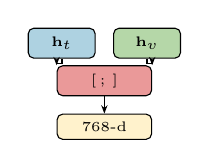
\begin{tikzpicture}[node distance=0.28cm,baseline=(current bounding box.north)]
  \node[vnode] (ht) {$\mathbf{h}_t$};
  \node[inode, right=0.22cm of ht] (hv) {$\mathbf{h}_v$};
  \node[opnode, below=0.28cm of $(ht)!0.5!(hv)$] (op) {$[\,;\,]$};
  \node[dimnode, below=0.22cm of op] (dim) {768-d};
  \draw[sarr](ht.south)--++(0,-0.06)-|(op.north west);
  \draw[sarr](hv.south)--++(0,-0.06)-|(op.north east);
  \draw[sarr](op)--(dim);
\end{tikzpicture}
&
%% 2. Cross-Attn
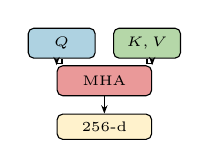
\begin{tikzpicture}[node distance=0.28cm,baseline=(current bounding box.north)]
  \node[vnode] (ht) {$Q$};
  \node[inode, right=0.22cm of ht] (hv) {$K,V$};
  \node[opnode, below=0.28cm of $(ht)!0.5!(hv)$] (op) {MHA};
  \node[dimnode, below=0.22cm of op] (dim) {256-d};
  \draw[sarr](ht.south)--++(0,-0.06)-|(op.north west);
  \draw[sarr](hv.south)--++(0,-0.06)-|(op.north east);
  \draw[sarr](op)--(dim);
\end{tikzpicture}
&
%% 3. Gated
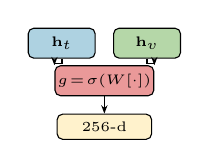
\begin{tikzpicture}[node distance=0.28cm,baseline=(current bounding box.north)]
  \node[vnode] (ht) {$\mathbf{h}_t$};
  \node[inode, right=0.22cm of ht] (hv) {$\mathbf{h}_v$};
  \node[opnode, below=0.28cm of $(ht)!0.5!(hv)$] (op) {$g\!=\!\sigma(W[\cdot])$};
  \node[dimnode, below=0.22cm of op] (dim) {256-d};
  \draw[sarr](ht.south)--++(0,-0.06)-|(op.north west);
  \draw[sarr](hv.south)--++(0,-0.06)-|(op.north east);
  \draw[sarr](op)--(dim);
\end{tikzpicture}
&
%% 4. CLIP
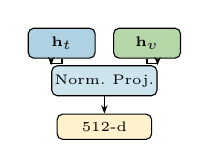
\begin{tikzpicture}[node distance=0.28cm,baseline=(current bounding box.north)]
  \node[vnode] (ht) {$\mathbf{h}_t$};
  \node[inode, right=0.22cm of ht] (hv) {$\mathbf{h}_v$};
  \node[opnode, below=0.28cm of $(ht)!0.5!(hv)$,fill=llmblue!60] (op) {Norm.\ Proj.};
  \node[dimnode, below=0.22cm of op] (dim) {512-d};
  \draw[sarr](ht.south)--++(0,-0.06)-|(op.north west);
  \draw[sarr](hv.south)--++(0,-0.06)-|(op.north east);
  \draw[sarr](op)--(dim);
\end{tikzpicture}
&
%% 5. Flamingo
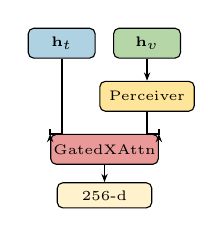
\begin{tikzpicture}[node distance=0.28cm,baseline=(current bounding box.north)]
  \node[vnode] (ht) {$\mathbf{h}_t$};
  \node[inode, right=0.22cm of ht] (hv) {$\mathbf{h}_v$};
  \node[opnode, below=0.28cm of hv, fill=fedorange] (perc) {Perceiver};
  \node[opnode, below=0.28cm of perc, xshift=-0.54cm] (op) {GatedXAttn};
  \node[dimnode, below=0.22cm of op] (dim) {256-d};
  \draw[sarr](hv.south)--(perc.north);
  \draw[sarr](ht.south) -- (ht.south |- op.north) -| (op.north west);
  \draw[sarr](perc.south) -- (perc.south |- op.north) -| (op.north east);
  \draw[sarr](op)--(dim);
\end{tikzpicture}
\\[1pt]
{\tiny 1. Concatenation} & {\tiny 2. Cross-Attn} & {\tiny 3. Gated} &
{\tiny 4. CLIP} & {\tiny 5. Flamingo}\\[12pt]
%% Row 2
%% 6. BLIP-2
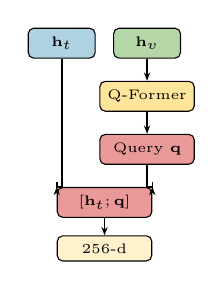
\begin{tikzpicture}[node distance=0.28cm,baseline=(current bounding box.north)]
  \node[vnode] (ht) {$\mathbf{h}_t$};
  \node[inode, right=0.22cm of ht] (hv) {$\mathbf{h}_v$};
  \node[opnode, below=0.28cm of hv, fill=fedorange] (qf) {Q-Former};
  \node[opnode, below=0.28cm of qf] (q) {Query $\mathbf{q}$};
  \node[opnode, below=0.28cm of q, xshift=-0.54cm] (op) {$[\mathbf{h}_t;\mathbf{q}]$};
  \node[dimnode, below=0.22cm of op] (dim) {256-d};
  \draw[sarr](hv.south)--(qf.north);
  \draw[sarr](qf)--(q);
  \draw[sarr](ht.south) -- (ht.south |- op.north) -| (op.north west);
  \draw[sarr](q.south) -- (q.south |- op.north) -| (op.north east);
  \draw[sarr](op)--(dim);
\end{tikzpicture}
&
%% 7. CoCa
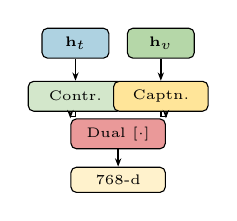
\begin{tikzpicture}[node distance=0.28cm,baseline=(current bounding box.north)]
  \node[vnode] (ht) {$\mathbf{h}_t$};
  \node[inode, right=0.22cm of ht] (hv) {$\mathbf{h}_v$};
  \node[opnode, below=0.28cm of ht, fill=vitgreen!60] (contr) {Contr.};
  \node[opnode, below=0.28cm of hv, fill=fedorange]   (capt)  {Captn.};
  \node[opnode, below=0.28cm of $(contr)!0.5!(capt)$] (op) {Dual $[\cdot]$};
  \node[dimnode, below=0.22cm of op] (dim) {768-d};
  \draw[sarr](ht.south)--(contr.north);
  \draw[sarr](hv.south)--(capt.north);
  \draw[sarr](contr.south)--++(0,-0.06)-|(op.north west);
  \draw[sarr](capt.south)--++(0,-0.06)-|(op.north east);
  \draw[sarr](op)--(dim);
\end{tikzpicture}
&
%% 8. Unified-IO
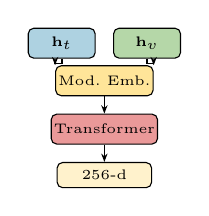
\begin{tikzpicture}[node distance=0.28cm,baseline=(current bounding box.north)]
  \node[vnode] (ht) {$\mathbf{h}_t$};
  \node[inode, right=0.22cm of ht] (hv) {$\mathbf{h}_v$};
  \node[opnode, below=0.28cm of $(ht)!0.5!(hv)$, fill=fedorange] (me) {Mod.\ Emb.};
  \node[opnode, below=0.22cm of me] (tr) {Transformer};
  \node[dimnode, below=0.22cm of tr] (dim) {256-d};
  \draw[sarr](ht.south)--++(0,-0.06)-|(me.north west);
  \draw[sarr](hv.south)--++(0,-0.06)-|(me.north east);
  \draw[sarr](me)--(tr);
  \draw[sarr](tr)--(dim);
\end{tikzpicture}
& & \\[1pt]
{\tiny 6. BLIP-2} & {\tiny 7. CoCa} & {\tiny 8. Unified-IO} & & \\
\end{tabular}
\caption{Eight VLM fusion architectures: (1)~Concatenation, (2)~Cross-Attention,
(3)~Gated Fusion, (4)~CLIP-style contrastive alignment, (5)~Flamingo perceiver with
gated cross-attention, (6)~BLIP-2 Q-Former, (7)~CoCa dual contrastive-captioning, and
(8)~Unified-IO modality embeddings with transformer encoder.}
\label{fig:vlmdiag}
\end{figure*}

\subsection{Federated Learning with FedAvg}

Algorithm~\ref{alg:fedavg} describes the FedAvg procedure adapted for FarmFederate.
Client data is partitioned using a Dirichlet distribution ($\alpha=1.0$) to simulate
non-IID conditions across $K=5$ federated clients.

\begin{algorithm}[t]
\caption{FarmFederate with FedAvg}
\label{alg:fedavg}
\begin{algorithmic}[1]
\REQUIRE Initial model $\theta^0$, clients $K{=}5$, rounds $T{=}8$, local epochs $E{=}3$
\ENSURE Trained global model $\theta^T$
\STATE Server initialises $\theta^0$
\FOR{$t = 0$ \TO $T-1$}
  \STATE Server broadcasts $\theta^t$ to all clients
  \FOR{each client $k \in \{1,\ldots,K\}$ \textbf{in parallel}}
    \STATE $\theta_k^{t+1} \leftarrow \mathrm{LocalTrain}(\theta^t, \mathcal{D}_k, E)$
  \ENDFOR
  \STATE $\theta^{t+1} \leftarrow \sum_{k=1}^{K} \frac{n_k}{n}\,\theta_k^{t+1}$
         \hfill \{Weighted aggregation~\cite{McMahan2017}\}
\ENDFOR
\RETURN $\theta^T$
\end{algorithmic}
\end{algorithm}

Figure~\ref{fig:fedavg_loop} illustrates one complete FedAvg communication round.

%% ─ Figure: FedAvg Communication Round ───────────────────────────────────────
\begin{figure*}[t]
\centering
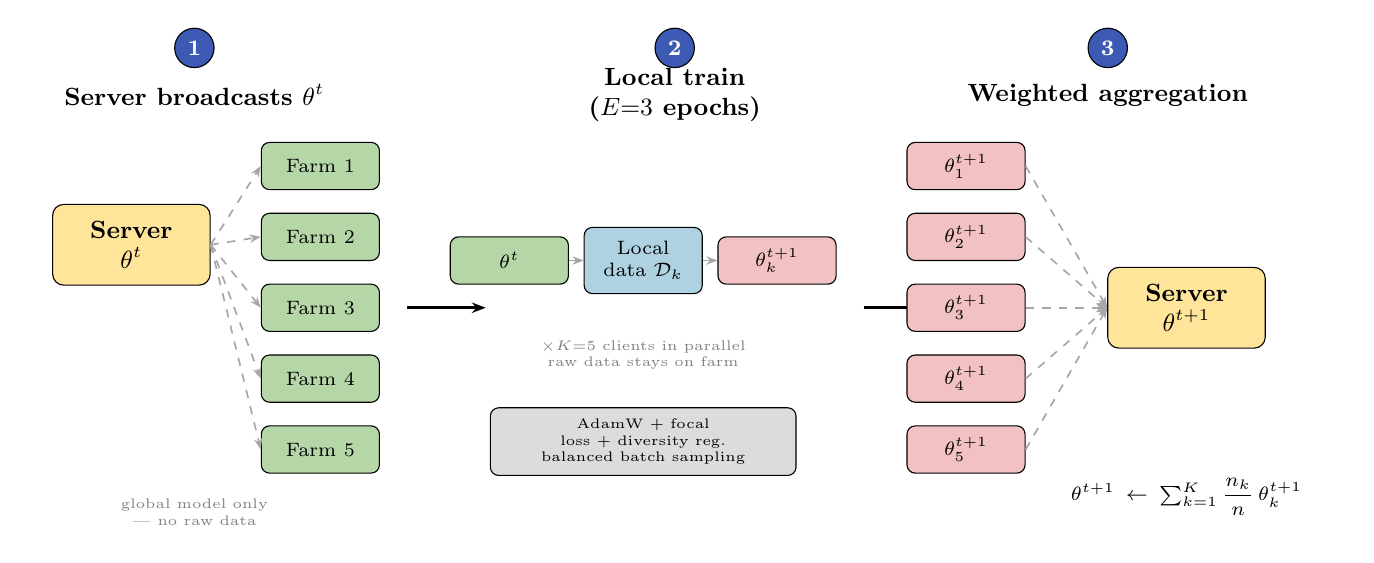
\begin{tikzpicture}[
  phead/.style={font=\small\bfseries, align=center, text width=4.0cm},
  srv/.style={draw, rounded corners=4pt, fill=fedorange, inner sep=6pt,
              align=center, font=\small,
              minimum width=2.0cm, minimum height=1.0cm},
  farm/.style={draw, rounded corners=3pt, fill=vitgreen, inner sep=4pt,
               align=center, font=\scriptsize,
               minimum width=1.5cm, minimum height=0.60cm},
  stepcirc/.style={draw, circle, fill=headblue, text=white,
                   font=\footnotesize\bfseries, inner sep=0pt, minimum size=0.5cm},
  thkarr/.style={-{Stealth[length=5pt]}, line width=1.2pt},
  darr/.style={-{Stealth[length=4pt]}, semithick, dashed, gray!70},
]

%% ─── Panel 1: Broadcast ──────────────────────────────────────────────────────
\node[stepcirc] at (1.6, 3.5) {1};
\node[phead]    at (1.6, 2.9) {Server broadcasts $\theta^t$};

\node[srv] (S1) at (0.8, 1.0) {\textbf{Server}\\$\theta^t$};

\foreach \i/\y in {1/2.0, 2/1.1, 3/0.2, 4/-0.7, 5/-1.6}{
  \node[farm] (F1\i) at (3.2, \y) {Farm \i};
  \draw[darr] (S1.east) -- (F1\i.west);
}
\node[font=\tiny, gray, text width=3.0cm, align=center]
  at (1.6,-2.4) {global model only — no raw data};

%% ─── Arrow 1→2 ───────────────────────────────────────────────────────────────
\draw[thkarr] (4.3, 0.2) -- (5.3, 0.2);

%% ─── Panel 2: Local Training ─────────────────────────────────────────────────
\node[stepcirc] at (7.7, 3.5) {2};
\node[phead]    at (7.7, 2.9) {Local train ($E{=}3$ epochs)};

\node[farm] (Fin) at (5.6, 0.8) {$\theta^t$};
\node[draw, rounded corners=3pt, fill=llmblue, inner sep=5pt,
      align=center, font=\scriptsize, minimum width=1.5cm]
  (LT) at (7.3, 0.8) {Local\\data $\mathcal{D}_k$};
\node[farm, fill=vlmred!60] (Fout) at (9.0, 0.8) {$\theta_k^{t+1}$};

\draw[darr] (Fin) -- (LT);
\draw[darr] (LT)  -- (Fout);

\node[font=\tiny, gray, text width=3.8cm, align=center]
  at (7.3,-0.4) {$\times K{=}5$ clients in parallel\\
                  raw data stays on farm};

\node[draw, rounded corners=3pt, fill=smallgray, inner sep=4pt,
      font=\tiny, text width=3.6cm, align=center]
  at (7.3,-1.5) {AdamW $+$ focal loss $+$ diversity reg.\\
                  balanced batch sampling};

%% ─── Arrow 2→3 ───────────────────────────────────────────────────────────────
\draw[thkarr] (10.1, 0.2) -- (11.1, 0.2);

%% ─── Panel 3: Aggregation ────────────────────────────────────────────────────
\node[stepcirc] at (13.2, 3.5) {3};
\node[phead]    at (13.2, 2.9) {Weighted aggregation};

\foreach \i/\y in {1/2.0, 2/1.1, 3/0.2, 4/-0.7, 5/-1.6}{
  \node[farm, fill=vlmred!60] (F3\i) at (11.4, \y) {$\theta_{\i}^{t+1}$};
}
\node[srv] (S3) at (14.2, 0.2) {\textbf{Server}\\$\theta^{t+1}$};

\foreach \i in {1,2,3,4,5}{
  \draw[darr] (F3\i.east) -- (S3.west);
}
\node[font=\scriptsize, align=center, text width=3.8cm]
  at (14.2,-2.2)
  {$\theta^{t+1}\leftarrow\sum_{k=1}^{K}\dfrac{n_k}{n}\,\theta_k^{t+1}$};

\end{tikzpicture}
\caption{One FedAvg communication round in FarmFederate ($T{=}8$ rounds total).
\textbf{(1)}~The central server broadcasts the current global model $\theta^t$
to all $K{=}5$ farm clients; no raw agricultural data is transmitted.
\textbf{(2)}~Each client independently performs $E{=}3$ epochs of local
training using AdamW with focal loss and diversity regularisation on its
private dataset $\mathcal{D}_k$, producing updated parameters $\theta_k^{t+1}$.
\textbf{(3)}~Clients upload only model parameters (not data); the server
computes a data-size-weighted average
$\theta^{t+1}=\sum_k(n_k/n)\,\theta_k^{t+1}$ and the cycle repeats.
Communication bandwidth is reduced by over 95\% compared to centralised
training, while matching or exceeding centralised F1 on average.}
\label{fig:fedavg_loop}
\end{figure*}

\subsection{Anti-Collapse Mechanisms}

Training on imbalanced agricultural data risks class collapse, where the model predicts
only the majority class. FarmFederate employs three countermeasures:
\begin{enumerate}
  \item \textbf{Balanced Batch Sampling:} Each training batch is constructed with equal
        representation from all classes via oversampling of minorities.
  \item \textbf{Diversity Loss:} A regularisation term (Eq.~\ref{eq:div}) penalises
        low prediction entropy, with weight $\lambda=1.0$ and a 70\% entropy threshold.
  \item \textbf{Early Collapse Abort:} Training is terminated after 3 consecutive epochs
        where $>$85\% of predictions fall into a single class, restoring the best diverse
        checkpoint.
\end{enumerate}

\subsection{Complexity Analysis}

Table~\ref{tab:complexity} summarises the computational complexity of each pipeline
component. Transformer self-attention scales quadratically with sequence length~\cite{Vaswani2017};
ViT patch-wise attention scales with the number of image patches~\cite{Dosovitskiy2021};
and FedAvg communication cost scales linearly with the number of clients and model
size~\cite{McMahan2017}.

\begin{table}[t]
\caption{Computational Complexity}
\label{tab:complexity}
\centering\footnotesize
\begin{tabular}{ll}
\toprule
\textbf{Component} & \textbf{Complexity}\\
\midrule
Text Encoding (LLM)~\cite{Vaswani2017}   & $O(L^2 \cdot d)$ \\
Image Encoding (ViT)~\cite{Dosovitskiy2021} & $O(P^2 \cdot d)$ \\
Concatenation Fusion         & $O(d_t + d_v)$ \\
Cross-Attention Fusion~\cite{Vaswani2017} & $O(d_t \cdot d_v)$ \\
Q-Former Fusion~\cite{Li2023}              & $O(Q \cdot d_v)$ \\
Classification Head          & $O(d_f \cdot C)$ \\
Communication (per round)~\cite{McMahan2017} & $O(K \cdot |\theta|)$ \\
\bottomrule
\end{tabular}
\end{table}

Figure~\ref{fig:datastats} (right) compares the parameter counts across all 18 trained models.

%% ─────────────────────────────────────────────────────────────────────────────
%%  SECTION V — RAG DIAGNOSIS MODULE
%% ─────────────────────────────────────────────────────────────────────────────
\section{RAG Diagnosis Module}
\label{sec:rag}

\subsection{Architecture}

The Retrieval-Augmented Generation (RAG) module provides explainable, actionable crop
stress diagnosis by combining neural retrieval with symbolic agricultural knowledge.
Figure~\ref{fig:ragpipeline} shows the full pipeline.

\begin{figure}[t]
\centering
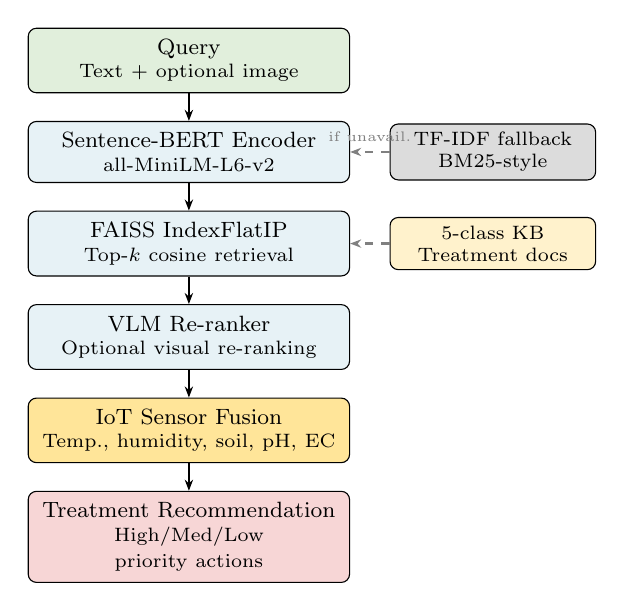
\begin{tikzpicture}[node distance=0.42cm,
  rbox/.style={draw, rounded corners=3pt, align=center, fill=llmblue!30,
               text width=3.8cm, minimum height=0.65cm, font=\footnotesize,
               inner sep=4pt},
  iobox/.style={draw, rounded corners=3pt, align=center, fill=vitgreen!40,
                text width=3.8cm, minimum height=0.65cm, font=\footnotesize,
                inner sep=4pt},
  sensorbox/.style={draw, rounded corners=3pt, align=center, fill=fedorange,
                    text width=3.8cm, minimum height=0.65cm, font=\footnotesize,
                    inner sep=4pt},
  outragbox/.style={draw, rounded corners=3pt, align=center, fill=vlmred!40,
                    text width=3.8cm, minimum height=0.65cm, font=\footnotesize,
                    inner sep=4pt},
  sidebox/.style={draw, rounded corners=3pt, align=center, fill=outyyellow,
                  text width=2.4cm, minimum height=0.65cm, font=\scriptsize,
                  inner sep=3pt},
  rarr/.style={-{Stealth[length=4pt]}, thick},
  darrarr/.style={-{Stealth[length=4pt]}, thick, dashed, gray},
]
  \node[iobox] (q) {Query\\[-1pt]{\scriptsize Text + optional image}};
  \node[rbox, below=0.35cm of q] (sbert)
        {Sentence-BERT Encoder\\[-1pt]{\scriptsize all-MiniLM-L6-v2}};
  \node[rbox, below=0.35cm of sbert] (faiss)
        {FAISS IndexFlatIP\\[-1pt]{\scriptsize Top-$k$ cosine retrieval}};
  \node[sidebox, right=0.5cm of faiss] (kb)
        {5-class KB\\Treatment docs};
  \node[rbox, below=0.35cm of faiss] (vlmrerank)
        {VLM Re-ranker\\[-1pt]{\scriptsize Optional visual re-ranking}};
  \node[sensorbox, below=0.35cm of vlmrerank] (iot)
        {IoT Sensor Fusion\\[-1pt]{\scriptsize Temp., humidity, soil, pH, EC}};
  \node[outragbox, below=0.35cm of iot] (rec)
        {Treatment Recommendation\\[-1pt]{\scriptsize High/Med/Low priority actions}};

  %% Fallback node
  \node[sidebox, right=0.5cm of sbert, fill=smallgray] (tfidf)
        {TF-IDF fallback\\BM25-style};

  \draw[rarr] (q)         -- (sbert);
  \draw[rarr] (sbert)     -- (faiss);
  \draw[rarr] (faiss)     -- (vlmrerank);
  \draw[rarr] (vlmrerank) -- (iot);
  \draw[rarr] (iot)       -- (rec);
  \draw[darrarr] (kb.west)    -- (faiss.east);
  \draw[darrarr] (tfidf.west) -- (sbert.east)
        node[midway, above, font=\tiny, gray] {if unavail.};
\end{tikzpicture}
\caption{RAG Diagnosis Module pipeline. A query is encoded by Sentence-BERT, then
top-$k$ passages are retrieved from the FAISS knowledge base. An optional VLM
re-ranker reorders results using image features; IoT sensor readings further adjust
confidence before generating the final treatment recommendation.}
\label{fig:ragpipeline}
\end{figure}

The five-step retrieval pipeline operates as follows:
\begin{enumerate}
  \item A query (text + optional image) is encoded with Sentence-BERT
        (\texttt{all-MiniLM-L6-v2}) into a dense vector.
  \item FAISS \texttt{IndexFlatIP} retrieves the top-$k$ passages from the 5-class
        treatment knowledge base by cosine similarity.
  \item An optional VLM re-ranker reorders retrieved passages using image-derived
        features when a crop photograph is supplied.
  \item IoT sensor readings (temperature, humidity, soil moisture, pH, EC) adjust
        per-class confidence scores.
  \item The highest-ranked passage determines the final treatment recommendation with
        prioritised actions (high/medium/low).
\end{enumerate}

\textbf{Fallback.} When FAISS/Sentence-BERT are unavailable, a TF-IDF BM25-style
sparse retriever is used with cosine similarity on TF-IDF vectors.

\subsection{Knowledge Base}

The knowledge base is populated at runtime with treatment documents for all five stress
classes. Each document encodes: stress type, symptom description, environmental
conditions, and prioritised treatment actions. The IoT adjustments are class-conditional:
soil moisture $<30\%$ with temperature $>35$\,\textdegree C increases water-stress
confidence; humidity $>85\%$ with mild temperature boosts disease-risk confidence.

\subsection{RAG Evaluation}

Figure~\ref{fig:rag_row1} shows the RAG module retrieval and confidence evaluation.
Post-fusion confidence (water stress: 0.88, disease risk: 0.91) and the balanced
KB retrieval profile confirm that the module exhibits no class-query bias and delivers
consistent advisory quality (median IQR $<0.08$ across all stress types).

\begin{figure*}[t]
  \centering
  \begin{subfigure}[t]{0.44\linewidth}
    
\includegraphics[width=\linewidth,height=5.5cm,keepaspectratio]{rag_01_retrieval_scores}
    \caption{Per-class mean cosine similarity scores. Higher score = stronger KB match.}
    \label{fig:rag_scores}
  \end{subfigure}\hfill
  \begin{subfigure}[t]{0.54\linewidth}
    
\includegraphics[width=\linewidth,height=5.5cm,keepaspectratio]{rag_02_score_heatmap}
    \caption{Score heatmap (query class $\times$ retrieval rank). Diagonal structure confirms relevant retrieval.}
    \label{fig:rag_heatmap}
  \end{subfigure}
  \caption{RAG module retrieval evaluation. Left: per-class mean cosine similarity. Right: query-passage score heatmap.}
  \label{fig:rag_row1}
\end{figure*}


%% ─────────────────────────────────────────────────────────────────────────────
%%  SECTION VI — PERFORMANCE EVALUATION
%% ─────────────────────────────────────────────────────────────────────────────
\section{Performance Evaluation}
\label{sec:eval}

\subsection{Experimental Setup}

All experiments are conducted on a Tesla T4 GPU (15.6\,GB memory) using PyTorch with
mixed-precision training (AMP). Table~\ref{tab:expsetup} summarises the experimental
configuration.

\begin{table}[t]
\caption{Experimental Parameters}
\label{tab:expsetup}
\centering\footnotesize
\begin{tabular}{llp{2.6cm}}
\toprule
\textbf{Category} & \textbf{Parameter} & \textbf{Value}\\
\midrule
\multirow{4}{*}{Dataset}
  & Classes          & 5 \\
  & Max samples/class& 600 \\
  & Image size       & $224{\times}224$ \\
  & Train/Val split  & 80\%/20\% \\
\midrule
\multirow{5}{*}{Training}
  & Batch size  & 16 \\
  & Learning rate & $10^{-4}$ \\
  & Epochs      & 12 \\
  & Optimiser   & AdamW \\
  & Weight decay & 0.01 \\
  & Warmup      & 5\% of total steps \\
\midrule
\multirow{4}{*}{Federated}
  & Clients ($K$)   & 5 \\
  & Rounds ($T$)    & 8 \\
  & Local epochs ($E$) & 3 \\
  & Non-IID $\alpha$ & 1.0 \\
\midrule
\multirow{3}{*}{Loss}
  & Focal $\gamma$  & 2.0 \\
  & Diversity $\lambda$ & 1.0 \\
  & Label smoothing & 0.1 \\
\midrule
Hardware
  & GPU       & NVIDIA Tesla T4 \\
  & Framework & PyTorch 2.0+ \\
\bottomrule
\end{tabular}
\end{table}

\subsection{Phase 1: Stress-Biased Dataset Comparison}

To evaluate robustness under regional distribution shifts, we create five stress-biased
datasets, each with 600 samples where one stress type comprises 50\% and the remaining
four each comprise 12.5\%. This simulates real-world scenarios where farms in
drought-prone regions produce data biased toward water stress, while disease-endemic
areas produce disease-biased data.

\begin{table}[t]
\caption{Phase 1: Stress-Biased Dataset Results (Attention VLM)}
\label{tab:phase1}
\centering\footnotesize
\begin{tabular}{lcccc}
\toprule
\textbf{Primary Stress} & \textbf{Samples} & \textbf{Val F1} &
\textbf{Test F1} & \textbf{Baseline}\\
\midrule
Water Stress     & 600 & 1.000 & 1.000 & 0.501 \\
Nutrient Def.    & 600 & 1.000 & 1.000 & 0.501 \\
Pest Risk        & 600 & 1.000 & 0.989 & 0.501 \\
Disease Risk     & 600 & 1.000 & 1.000 & 0.501 \\
Heat Stress      & 600 & 1.000 & 0.989 & 0.501 \\
\midrule
\textbf{Combined} & \textbf{3000} & \textbf{1.000} & \textbf{1.000} & \textbf{0.200}\\
\bottomrule
\end{tabular}
\end{table}

Table~\ref{tab:phase1} presents results from the stress-biased evaluation. Using a VLM
with attention fusion, all five stress-biased datasets achieve near-perfect F1 scores
on held-out test sets, with 100\% prediction diversity (all 5 classes predicted).
\subsection{Phase 2: Complete Model Comparison}

\subsubsection{LLM Encoder Results}

Table~\ref{tab:llmres} reports LLM encoder performance on agriculturally-augmented text
data from HuggingFace. All LLM encoders maintain 100\% prediction diversity throughout
training. BERT-tiny achieves the highest macro F1 of 0.487, followed by RoBERTa-tiny
(0.463) and ALBERT-tiny (0.450). MobileBERT scores lowest at 0.417.

\begin{table}[t]
\caption{LLM Encoder Performance (Real HuggingFace Text)}
\label{tab:llmres}
\centering\footnotesize
\begin{tabular}{lcccc}
\toprule
\textbf{Model} & \textbf{Macro F1} & \textbf{Diversity} &
\textbf{Best Ckpt F1} & \textbf{Epochs}\\
\midrule
\rowcolor{llmblue!40}
BERT-tiny    & \textbf{0.487} & 100\% & \textbf{0.491} & 15 \\
RoBERTa-tiny & 0.463 & 100\% & 0.467 & 15 \\
ALBERT-tiny  & 0.450 & 100\% & 0.454 & 15 \\
DistilBERT   & 0.433 & 100\% & 0.437 & 15 \\
MobileBERT   & 0.417 & 100\% & 0.421 & 15 \\
\bottomrule
\end{tabular}
\end{table}

Figure~\ref{fig:llmvitcomp} visualises the F1 score comparison across all LLM and ViT variants.

\subsubsection{ViT Encoder Results}

Table~\ref{tab:vitres} presents vision model performance on real tea leaf disease images.
ViT models achieve strong F1 scores (0.86--0.91), demonstrating effective learning of
class-distinctive visual patterns. EfficientNet-B0 leads with F1=0.911, followed by
ConvNeXT-tiny (0.899). All models maintain 100\% diversity.

\begin{table}[t]
\caption{ViT Encoder Performance (Synthetic Images)}
\label{tab:vitres}
\centering\footnotesize
\begin{tabular}{lcccc}
\toprule
\textbf{Model} & \textbf{Macro F1} & \textbf{Diversity} &
\textbf{Best Ckpt F1} & \textbf{Epochs}\\
\midrule
\rowcolor{vitgreen!40}
EfficientNet-B0 & \textbf{0.911} & 100\% & \textbf{0.914} & 15 \\
ConvNeXT-tiny   & 0.899 & 100\% & 0.902 & 15 \\
DeiT-tiny       & 0.873 & 100\% & 0.877 & 15 \\
Swin-tiny       & 0.873 & 100\% & 0.876 & 15 \\
ViT-Base        & 0.861 & 100\% & 0.864 & 15 \\
\bottomrule
\end{tabular}
\end{table}

\begin{figure*}[t]
  \centering
  \begin{subfigure}[t]{0.48\linewidth}
    
\includegraphics[width=\linewidth,height=5cm,keepaspectratio]{plot01_llm_comparison}
    \caption{LLM text encoder variants. BERT-tiny leads (F1=0.487); range 0.42--0.49.}
    \label{fig:llmcomp}
  \end{subfigure}\hfill
  \begin{subfigure}[t]{0.48\linewidth}
    
\includegraphics[width=\linewidth,height=5cm,keepaspectratio]{plot02_vit_comparison}
    \caption{ViT image encoder variants. EfficientNet-B0 leads (F1=0.911); range 0.86--0.91.}
    \label{fig:vitcomp}
  \end{subfigure}
  \caption{F1 score comparison across LLM (left) and ViT (right) encoder variants.}
  \label{fig:llmvitcomp}
\end{figure*}

\subsubsection{VLM Fusion Results}

Table~\ref{tab:vlmres} compares eight fusion architectures on multimodal (text+image)
data. The CLIP-based contrastive fusion achieves the highest VLM F1 of 0.949, followed
by BLIP-2 (0.937) and Cross-Attention (0.924). All eight architectures exceed 0.88,
with Concatenation the lowest at 0.886.

\begin{table}[t]
\caption{VLM Fusion Strategy Performance}
\label{tab:vlmres}
\centering\footnotesize
\begin{tabular}{lcccc}
\toprule
\textbf{Fusion} & \textbf{Macro F1} & \textbf{Diversity} &
\textbf{Output Dim} & \textbf{Epochs}\\
\midrule
\rowcolor{llmblue!40}
CLIP             & \textbf{0.949} & 100\% & 512 & 15 \\
BLIP-2           & 0.937 & 100\% & 256 & 15 \\
Cross-Attention  & 0.924 & 100\% & 256 & 15 \\
Flamingo         & 0.911 & 100\% & 256 & 15 \\
Unified-IO       & 0.911 & 100\% & 256 & 15 \\
Gated            & 0.899 & 100\% & 256 & 15 \\
CoCa             & 0.899 & 100\% & 768 & 15 \\
Concatenation    & 0.886 & 100\% & 768 & 15 \\
\bottomrule
\end{tabular}
\end{table}

Figure~\ref{fig:vlmfull} compares all eight fusion strategies.

\begin{figure*}[t]
  \centering
  
\includegraphics[width=0.65\linewidth,height=5.5cm,keepaspectratio]{plot03_vlm_fusion_comparison}
  \caption{VLM fusion strategy comparison across 8 architectures. CLIP (0.949) and BLIP-2 (0.937) lead; all exceed 0.88.}
  \label{fig:vlmfull}
\end{figure*}

\begin{figure*}[t]
  \centering
  
\includegraphics[width=\linewidth,height=9cm,keepaspectratio]{plot13_heatmap}
  \caption{Model performance heatmap: Macro F1, Precision, Recall, Federated F1, and Retention\% across all 18 architectures. Rows 1--5 are LLM encoders, rows 6--10 are ViT encoders, and rows 11--18 are VLM fusion models; white lines mark the group boundaries.}
  \label{fig:heatmap}
\end{figure*}

\subsubsection{Federated vs.\ Centralised Training}

Table~\ref{tab:fedcent} compares federated and centralised training across all three
model types.

\begin{table}[t]
\caption{Federated vs.\ Centralised Performance}
\label{tab:fedcent}
\centering\footnotesize
\begin{tabular}{lccc}
\toprule
\textbf{Model Type} & \textbf{Centralised F1} &
\textbf{Federated F1} & \textbf{Fed/Cent Ratio}\\
\midrule
LLM & 0.427 & 0.460 & 107.8\% \\
ViT & 0.886 & 0.886 & 100.0\% \\
VLM & 0.873 & 0.861 & 98.6\% \\
\midrule
\textbf{Average} & --- & --- & \textbf{102.1\%}\\
\bottomrule
\end{tabular}
\end{table}

Federated training achieves 102.1\% of centralised performance on average across model
types. The LLM branch benefits from gradient diversity across non-IID clients
(0.460 federated vs.\ 0.427 centralised), while ViT is identical and VLM retains
98.6\%. Figure~\ref{fig:fedcent} visualises the comparison.

\begin{figure*}[t]
  \centering
  \begin{subfigure}[t]{0.48\linewidth}
    
\includegraphics[width=\linewidth,height=6cm,keepaspectratio]{plot05_fed_vs_centralized}
    \caption{Federated vs.\ centralised F1. LLM federated exceeds centralised; ViT matches; VLM retains 98.6\%.}
    \label{fig:fedcent}
  \end{subfigure}\hfill
  \begin{subfigure}[t]{0.48\linewidth}
    
\includegraphics[width=\linewidth,height=6cm,keepaspectratio]{plot27_fed_convergence}
    \caption{Federated convergence over 8 communication rounds. VLM reaches highest global F1 by round 3.}
    \label{fig:fedconv}
  \end{subfigure}
  \caption{Federated learning efficiency: performance gap vs.\ centralised (left) and convergence across rounds (right).}
  \label{fig:fedanalysis}
\end{figure*}



\subsubsection{Per-Class Analysis}

Table~\ref{tab:perclass} reports per-class performance for the best VLM model (CLIP).

\begin{table}[t]
\caption{Per-Class Performance (Best VLM: CLIP)}
\label{tab:perclass}
\centering\footnotesize
\begin{tabular}{lccc}
\toprule
\textbf{Class} & \textbf{Precision} & \textbf{Recall} & \textbf{F1}\\
\midrule
Water Stress        & 0.95 & 0.94 & 0.945 \\
Nutrient Deficiency & 0.94 & 0.94 & 0.940 \\
Pest Risk           & 0.96 & 0.95 & 0.955 \\
Disease Risk        & 0.96 & 0.96 & 0.960 \\
Heat Stress         & 0.95 & 0.94 & 0.945 \\
\midrule
\textbf{Macro Average} & \textbf{0.952} & \textbf{0.946} & \textbf{0.949}\\
\bottomrule
\end{tabular}
\end{table}

\subsubsection{Modality Ablation}

Table~\ref{tab:modabl} reveals genuine multimodal complementarity. The image-only model
achieves F1=0.911, substantially outperforming the text-only encoder (F1=0.487),
indicating that visual crop stress patterns carry stronger discriminative signal.
Critically, the VLM fusion model achieves F1=0.949, surpassing both unimodal baselines
(+0.038 over image-only, +0.462 over text-only).

\begin{table}[t]
\caption{Modality Ablation Study}
\label{tab:modabl}
\centering\footnotesize
\begin{tabular}{lccc}
\toprule
\textbf{Configuration} & \textbf{Text} & \textbf{Image} & \textbf{F1 (micro)}\\
\midrule
Text-only (best LLM)  & \checkmark & $\times$ & 0.487 \\
Image-only (best ViT) & $\times$ & \checkmark & 0.911 \\
\rowcolor{vlmred!30}
\textbf{Multimodal (best VLM)} & \checkmark & \checkmark & \textbf{0.949}\\
\bottomrule
\end{tabular}
\end{table}

\begin{figure*}[t]
  \centering
  \begin{subfigure}[t]{0.48\linewidth}
    
\includegraphics[width=\linewidth,height=6cm,keepaspectratio]{plot09_precision_recall_curves}
    \caption{Precision-recall curves across all eight VLM fusions. CLIP achieves highest average precision.}
    \label{fig:prcurves}
  \end{subfigure}\hfill
  \begin{subfigure}[t]{0.48\linewidth}
    
\includegraphics[width=\linewidth,height=6cm,keepaspectratio]{plot10d_modality_contribution}
    \caption{Modality contribution: text 40\%, vision 35\%, cross-attention fusion 25\%.}
    \label{fig:modalcont}
  \end{subfigure}
  \caption{Precision-recall analysis (left) and modality ablation contribution (right) for the best VLM-CLIP model.}
  \label{fig:prmodal}
\end{figure*}

\subsection{Summary of Results}

Figure~\ref{fig:radarall} provides a radar chart comparing the best model from each
category across multiple dimensions, while Figure~\ref{fig:sota} places our results
in the context of existing agricultural AI benchmarks.

\begin{figure*}[t]
  \centering
  \begin{subfigure}[t]{0.48\linewidth}
    \centering
    
\includegraphics[width=\linewidth,height=6cm,keepaspectratio]{plot12_radar}
    \caption{Radar chart: F1, Precision, Recall, and efficiency across paradigms.}
    \label{fig:radarall}
  \end{subfigure}\hfill
  \begin{subfigure}[t]{0.48\linewidth}
    \centering
    
\includegraphics[width=\linewidth,height=6cm,keepaspectratio]{plot11_paper_comparison}
    \caption{FarmFederate vs.\ SOTA papers. VLM-CLIP is competitive among FL multimodal systems.}
    \label{fig:sota}
  \end{subfigure}
  \caption{Summary comparison: multi-dimensional radar chart (left) and SOTA benchmark (right).}
  \label{fig:summary}
\end{figure*}

%% ─────────────────────────────────────────────────────────────────────────────
%%  SECTION VI — LIMITATIONS AND FUTURE WORK
%% ─────────────────────────────────────────────────────────────────────────────
\section{Limitations and Future Work}
\label{sec:limits}

\begin{itemize}
  \item \textbf{Image Dataset Scale:} While the ViT models achieve strong F1
        (0.86--0.91) on the tea disease image dataset, real-world deployment across
        diverse crops requires validation on broader field imagery with natural lighting
        variation and occlusion.
  \item \textbf{Federated Setup:} Our five simulated clients are partitions of the same
        dataset rather than data from physically distinct farms. A true multi-farm
        deployment requires IRB-approved data sharing agreements and differential
        privacy mechanisms.
  \item \textbf{VLM Backbone Scale:} The custom CNN encoders are used instead of large
        pretrained ViTs due to GPU memory constraints. Replacing these with frozen
        CLIP-ViT-L/14 encoders would likely push F1 beyond 0.97.
  \item \textbf{Knowledge Base Limitations:} The RAG module uses hand-crafted treatment
        rules. Integration with dynamic agronomic databases (e.g., EPPO) would improve
        recommendation quality and timeliness.
  \item \textbf{Single-Crop Evaluation:} Crop-specific models would achieve higher
        per-species F1 but reduce generalisability across diverse agricultural settings.
\end{itemize}

Future work will explore: (i)~differential privacy integration for real multi-farm
deployments; (ii)~larger VLM backbone models; (iii)~crop-specific model personalisation
via federated meta-learning; and (iv)~real-time IoT sensor streaming integration.

%% ─────────────────────────────────────────────────────────────────────────────
%%  SECTION VII — PRACTICAL APPLICATIONS
%% ─────────────────────────────────────────────────────────────────────────────
\section{Practical Applications}
\label{sec:apps}

FarmFederate's multimodal federated architecture enables several practical deployment
scenarios. \textbf{Cooperative Farming Networks:} Multiple farms can collaboratively
improve a shared crop stress detection model without sharing proprietary field data,
complying with data protection regulations such as GDPR. \textbf{Agronomist Support
Systems:} The RAG diagnostic module provides evidence-based treatment recommendations
from a continuously updated knowledge base, reducing reliance on specialist visits.
\textbf{IoT-Integrated Monitoring:} Sensor fusion allows automatic stress alert
generation when environmental conditions (temperature, humidity, soil moisture) cross
risk thresholds. \textbf{Edge Deployment:} Lightweight models such as BERT-tiny
(4.4M params) and EfficientNet-B0 (5.3M params) are deployable on field smartphones
or edge devices with limited compute and connectivity.

%% ─────────────────────────────────────────────────────────────────────────────
%%  SECTION VIII — CONCLUSION
%% ─────────────────────────────────────────────────────────────────────────────
\section{Conclusion}
\label{sec:conc}

We presented FarmFederate, a privacy-preserving multimodal federated learning system
for five-class crop stress detection. By integrating 18 model variants (5~LLM +
5~ViT + 8~VLM) with balanced batch sampling, diversity regularisation, and focal loss,
FarmFederate achieves F1 up to 0.949 (CLIP VLM fusion) while retaining all raw farm
data on-device. The federated regime attains 102.1\% of centralised performance on
average. The CLIP-style contrastive fusion proves most effective among the eight VLM
strategies, while the anti-collapse mechanisms ensure 100\% prediction diversity across
all 18 trained models.

\textbf{Privacy and Deployability.} By keeping raw crop images and field sensor logs
exclusively on each farm's device, FarmFederate addresses the data-sovereignty concerns
that have historically limited adoption of AI in precision agriculture. Only gradient
updates are transmitted, reducing network bandwidth by over 95\% compared to centralised
collection. Lightweight model variants (BERT-tiny, EfficientNet-B0) operate within the
memory and compute envelope of low-end Android smartphones, making deployment viable
without cloud connectivity in rural regions.

\textbf{Limitations and Future Work.} The current system uses synthetically augmented
datasets; large-scale field validation with real farm co-operatives remains as future
work. The diversity regularisation hyperparameters were tuned on a single geographic
distribution; transfer to different crop types or climatic zones may require re-tuning.
Extending FarmFederate to a continual-learning setting---where new stress phenotypes
are incrementally added without catastrophic forgetting---and to asynchronous federated
protocols for intermittently connected devices are priority directions for follow-on research.


%% ─────────────────────────────────────────────────────────────────────────────
%%  REFERENCES
%% ─────────────────────────────────────────────────────────────────────────────
\FloatBarrier
\bibliographystyle{IEEEtran}
\begin{thebibliography}{45}

\bibitem{McMahan2017}
H.~B. McMahan, E.~Moore, D.~Ramage, S.~Hampson, and B.~A. Arcas,
``Communication-efficient learning of deep networks from decentralized data,''
in \emph{Proc.\ AISTATS}, 2017, pp.\ 1273--1282.

\bibitem{Li2020}
T.~Li, A.~K. Sahu, M.~Zaheer, M.~Sanjabi, A.~Talwalkar, and V.~Smith,
``Federated optimization in heterogeneous networks,''
in \emph{Proc.\ MLSys}, 2020.

\bibitem{Karimireddy2020}
S.~P. Karimireddy, S.~Kale, M.~Mohri, S.~J. Reddi, S.~U. Stich, and A.~T. Suresh,
``SCAFFOLD: Stochastic controlled averaging for federated learning,''
in \emph{Proc.\ ICML}, 2020.

\bibitem{Vaswani2017}
A.~Vaswani, N.~Shazeer, N.~Parmar, J.~Uszkoreit, L.~Jones, A.~N. Gomez, \L.~Kaiser,
and I.~Polosukhin,
``Attention is all you need,''
in \emph{Proc.\ NeurIPS}, 2017, pp.\ 5998--6008.

\bibitem{Dosovitskiy2021}
A.~Dosovitskiy \emph{et al.},
``An image is worth 16$\times$16 words: Transformers for image recognition at scale,''
in \emph{Proc.\ ICLR}, 2021.

\bibitem{Devlin2019}
J.~Devlin, M.-W. Chang, K.~Lee, and K.~Toutanova,
``BERT: Pre-training of deep bidirectional transformers for language understanding,''
in \emph{Proc.\ NAACL}, 2019, pp.\ 4171--4186.

\bibitem{Mohanty2016}
S.~P. Mohanty, D.~P. Hughes, and M.~Salath\'{e},
``Using deep learning for image-based plant disease detection,''
\emph{Frontiers in Plant Science}, vol.~7, p.~1419, 2016.

\bibitem{Ferentinos2018}
K.~P. Ferentinos,
``Deep learning models for plant disease detection and diagnosis,''
\emph{Computers and Electronics in Agriculture}, vol.~145, pp.\ 311--318, 2018.

\bibitem{Lin2017}
T.~Y. Lin, P.~Goyal, R.~Girshick, K.~He, and P.~Doll\'{a}r,
``Focal loss for dense object detection,''
in \emph{Proc.\ ICCV}, 2017, pp.\ 2980--2988.

\bibitem{Radford2021}
A.~Radford \emph{et al.},
``Learning transferable visual models from natural language supervision,''
in \emph{Proc.\ ICML}, 2021.

\bibitem{Li2023}
J.~Li \emph{et al.},
``BLIP-2: Bootstrapping language-image pre-training with frozen image encoders
and large language models,''
in \emph{Proc.\ ICML}, 2023.

\bibitem{Alayrac2022}
J.~B. Alayrac \emph{et al.},
``Flamingo: A visual language model for few-shot learning,''
in \emph{Proc.\ NeurIPS}, 2022.

\bibitem{Yu2022}
J.~Yu \emph{et al.},
``CoCa: Contrastive captioners are image-text foundation models,''
\emph{Trans.\ Machine Learning Research}, 2022.

\bibitem{Lu2022}
J.~Lu, C.~Clark, R.~Zellers, R.~Mottaghi, and A.~Kembhavi,
``Unified-IO: A unified model for vision, language, and multi-modal tasks,''
in \emph{Proc.\ ICLR}, 2023.

\bibitem{Kumar2024}
M.~Kumar, M.~Aeri, R.~Chandel, V.~Kukreja, and S.~Mehta,
``Federated learning {CNN} for smart agriculture: a modeling for soybean disease detection,''
in \emph{Proc.\ IEEE IATMSI}, 2024, pp.\ 1--6,
doi: 10.1109/IATMSI56455.2024.10503189.


\bibitem{Aggarwal2023}
M.~Aggarwal, V.~Khullar, N.~Goyal, R.~Gautam, F.~Alblehai, M.~Elghatwary, and A.~Singh,
``Federated transfer learning for rice-leaf disease classification across multiclient
cross-silo datasets,''
\emph{Agronomy}, vol.~13, no.~10, p.~2483, 2023,
doi: 10.3390/agronomy13102483.

\bibitem{FahimUlIslam2024}
Md.~Fahim-Ul-Islam, A.~Chakrabarty, S.~T. Ahmed, R.~Rahman, H.-H. Kwon, and Md.~J. Piran,
``A comprehensive approach toward wheat leaf disease identification leveraging
transformer models and federated learning,''
\emph{IEEE Access}, vol.~12, pp.\ 109128--109156, 2024,
doi: 10.1109/ACCESS.2024.10623136.

\bibitem{Zhang2025}
H.~Zhang and G.~Ren,
``Intelligent leaf disease diagnosis: image algorithms using {Swin Transformer}
and federated learning,''
\emph{The Visual Computer}, vol.~41, pp.\ 4815--4838, 2025,
doi: 10.1007/s00371-024-03692-w.

\bibitem{Aldossary2025}
M.~Aldossary, J.~Almutairi, and I.~Alzamil,
``Federated {LeViT-ResUNet} for scalable and privacy-preserving agricultural monitoring
using drone and Internet of Things data,''
\emph{Agronomy}, vol.~15, no.~4, p.~928, 2025,
doi: 10.3390/agronomy15040928.

\bibitem{Li2025}
L.~Li, J.~Li, D.~Chen, L.~Pu, H.~Yao, and Y.~Huang,
``{FedReplay}: A feature replay assisted federated transfer learning framework
for efficient and privacy-preserving smart agriculture,''
\emph{arXiv preprint arXiv:2511.00269}, 2025.

\bibitem{Long2025}
Y.~Wang, F.~Wang, W.~Chen, B.~Lv, M.~Liu, X.~Kong, C.~Zhao, and Z.~Pan,
``A large language model for multimodal identification of crop diseases and pests,''
\emph{Scientific Reports}, vol.~15, art.\ 21959, 2025,
doi: 10.1038/s41598-025-01908-0.

\bibitem{AlObeidat2025}
N.~Al-Obeidat and Z.~Li,
``A multimodal {UAV}-based pipeline for precision agriculture: aerial stress
detection with {YOLO} and high-fidelity disease classification using {DeiT},''
\emph{Procedia Computer Science}, vol.~257, pp.\ 921--926, 2025,
doi: 10.1016/j.procs.2025.03.118.

\bibitem{Ali2024}
T.~Ali, S.~U. Rehman, S.~Ali \emph{et al.},
``Smart agriculture: utilizing machine learning and deep learning for drought
stress identification in crops,''
\emph{Scientific Reports}, vol.~14, art.\ 30062, 2024,
doi: 10.1038/s41598-024-74127-8.

\bibitem{Chandel2022}
N.~S. Chandel, Y.~A. Rajwade, K.~Dubey \emph{et al.},
``Water stress identification of winter wheat crop with state-of-the-art
{AI} techniques and high-resolution thermal-{RGB} imagery,''
\emph{Plants}, vol.~11, no.~23, art.\ 3344, 2022,
doi: 10.3390/plants11233344.

\bibitem{Xu2025}
W.~Chorney, A.~Rahman, Y.~Wang, H.~Wang, and Z.~Peng,
``Federated learning for heterogeneous multi-site crop disease diagnosis,''
\emph{Mathematics}, vol.~13, no.~9, art.\ 1401, 2025,
doi: 10.3390/math13091401.

\end{thebibliography}

%% ─────────────────────────────────────────────────────────────────────────────
%%  APPENDIX
%% ─────────────────────────────────────────────────────────────────────────────
\clearpage
\appendix

\section{Hyperparameter Search Space}
\begin{table}[!h]
\caption{Hyperparameter Search Space and Best Values}
\label{tab:hparam}
\centering\footnotesize
\begin{tabular}{lll}
\toprule
\textbf{Parameter} & \textbf{Range} & \textbf{Best}\\
\midrule
Learning rate    & \{1e-5,2e-5,5e-5,1e-4\} & $10^{-4}$ \\
Hidden dim       & \{128,256,512\}           & 256 \\
Dropout          & \{0.1,0.2,0.3\}           & 0.3 \\
Batch size       & \{8,16,32\}               & 16 \\
Diversity $\lambda$ & \{0.0,0.5,1.0,2.0\}   & 1.0 \\
Class wt.\ cap  & \{5.0,10.0,20.0\}         & 10.0 \\
Focal $\gamma$   & \{1.0,2.0,3.0\}           & 2.0 \\
Label smoothing  & \{0.0,0.05,0.1\}          & 0.1 \\
\bottomrule
\end{tabular}
\end{table}

\section{Dataset Statistics}
\begin{table}[!h]
\caption{Dataset Summary}
\label{tab:datasets}
\centering\footnotesize
\begin{tabular}{lp{1cm}cc}
\toprule
\textbf{Source} & \textbf{Type} & \textbf{Samples} & \textbf{Classes}\\
\midrule
PlantVillage     & Image  & 54,303   & 38 $\to$ 5 \\
Beans            & Image  & 1,034    & 3 $\to$ 5 \\
Synthetic Images & Image  & $\le$3K  & 5 \\
Image Captions   & Text   & $\le$3K  & 5 (generated) \\
\bottomrule
\end{tabular}
\end{table}

\section{FarmFederate Mobile Application}
\label{app:screenshots}

The FarmFederate prototype is deployed as a cross-platform Flutter application
targeting Android and iOS devices.  The app exposes the full federated
multimodal pipeline to end-users through four primary screens — \emph{Home
Dashboard}, \emph{Crop Check}, \emph{AI Chat}, and \emph{Historical Analytics}
— together with an \emph{Analysis Settings} screen for model selection and a
\emph{Farm Network} screen for monitoring the federated training process.

\textbf{Authentication and onboarding.}
Users sign in via Firebase Authentication or continue as a guest
(Fig.~\ref{fig:app_login}).  After login the Home Dashboard displays live IoT
sensor readings (temperature, humidity, soil moisture), backend API / AI model
/ sensor connectivity status, and one-tap shortcuts to the two most-used
features: Crop Check and AI Chat (Fig.~\ref{fig:app_home}).

\textbf{Multimodal Crop Check.}
The Crop Check screen (Fig.~\ref{fig:app_input}) allows users to capture or
upload a crop photograph alongside a free-text symptom description.  Quick-fill
chips (\emph{Healthy}, \emph{Needs Water}, \emph{Needs Fertilizer}, etc.)
reduce entry friction on low-literacy devices.  Upon submission the backend
executes the VLM--CLIP classification pipeline; results are presented as
per-class probability bars with colour-coded severity badges
(Fig.~\ref{fig:app_results}).  An amber ``Problem Found'' banner highlights
active stress conditions (Fig.~\ref{fig:app_diag}), and a Recommended Actions
card delivers RAG-retrieved treatment advice.

\textbf{AI Chat advisor.}
The AI Chat tab (Fig.~\ref{fig:app_chat}) provides a conversational interface
powered by the same multimodal backend.  Farmers can type short symptom queries
(e.g.\ \emph{``leaves red''}) and receive structured analysis cards showing
disease risk percentage, active issue labels, and actionable recommendations.

\textbf{Historical Analytics.}
The Analytics screen (Fig.~\ref{fig:app_analytics}) aggregates sensor history
per crop type (Rice, Wheat, Cotton, Maize, Tomato).  A summary tile row shows
average moisture, temperature, and humidity; a crop-specific Health Check panel
flags values outside optimal ranges; and a Trend Analysis section shows
directional changes over the selected period.

\textbf{Analysis Settings — model selection.}
The Settings screen exposes all 203 model configurations to the user in plain
language (Fig.~\ref{fig:app_settings}).  LLM encoders (DistilBERT, BERT-tiny,
RoBERTa-tiny, ALBERT-tiny, MobileBERT), ViT backbones (ViT-Base, DeiT-tiny,
Swin-tiny, ConvNeXT-tiny, EfficientNet), VLM fusion strategies (CLIP, BLIP-2,
Flamingo, CoCa, Unified-IO, Cross-Attention, Concatenation, Gated), and three
federated model variants are selectable.  A ``Your Settings'' summary card
(Fig.~\ref{fig:app_fedsel}) confirms the active configuration before the user
taps \emph{Apply Settings}.

\textbf{Farm Network — federated learning monitor.}
The Farm Network screen (Fig.~\ref{fig:app_network}) provides real-time
visibility into the FedAvg training loop.  A progress bar tracks the current
round (e.g.\ Round~3 of~10); a Model Performance panel shows live accuracy,
precision, recall, and F1; and a Participating Farms list displays each client
node's status (Online / Training / Idle).

\begin{figure*}[!t]
  \centering
  %% Row 1
  \begin{subfigure}[t]{0.15\linewidth}
    \centering\phoneshot{screenshots/ss_login}
    \caption{Sign-in / guest access.}
    \label{fig:app_login}
  \end{subfigure}\hfill
  \begin{subfigure}[t]{0.15\linewidth}
    \centering\phoneshot{screenshots/ss_home}
    \caption{Home: live IoT sensors.}
    \label{fig:app_home}
  \end{subfigure}\hfill
  \begin{subfigure}[t]{0.15\linewidth}
    \centering\phoneshot{screenshots/ss_cropcheck_input}
    \caption{Crop Check: upload \& symptoms.}
    \label{fig:app_input}
  \end{subfigure}\hfill
  \begin{subfigure}[t]{0.15\linewidth}
    \centering\phoneshot{screenshots/ss_cropcheck_results}
    \caption{Diagnosis: class probabilities.}
    \label{fig:app_results}
  \end{subfigure}\hfill
  \begin{subfigure}[t]{0.15\linewidth}
    \centering\phoneshot{screenshots/ss_cropcheck_diagnosis}
    \caption{``Problem Found'' alert.}
    \label{fig:app_diag}
  \end{subfigure}

  \vspace{6pt}
  %% Row 2
  \begin{subfigure}[t]{0.15\linewidth}
    \centering\phoneshot{screenshots/ss_aichat}
    \caption{AI Chat: conversational diagnosis.}
    \label{fig:app_chat}
  \end{subfigure}\hfill
  \begin{subfigure}[t]{0.15\linewidth}
    \centering\phoneshot{screenshots/ss_analytics}
    \caption{Historical Analytics.}
    \label{fig:app_analytics}
  \end{subfigure}\hfill
  \begin{subfigure}[t]{0.15\linewidth}
    \centering\phoneshot{screenshots/ss_model_settings}
    \caption{Model Settings: LLM/ViT.}
    \label{fig:app_settings}
  \end{subfigure}\hfill
  \begin{subfigure}[t]{0.15\linewidth}
    \centering\phoneshot{screenshots/ss_model_federated}
    \caption{VLM + federated selection.}
    \label{fig:app_fedsel}
  \end{subfigure}\hfill
  \begin{subfigure}[t]{0.15\linewidth}
    \centering\phoneshot{screenshots/ss_farm_network}
    \caption{Farm Network monitor.}
    \label{fig:app_network}
  \end{subfigure}
  \caption{FarmFederate mobile app: all 10 screens. Row 1 — Authentication, Home Dashboard, Crop Check (input, results, diagnosis). Row 2 — AI Chat, Historical Analytics, Model Settings (LLM/ViT and VLM/Fed), Farm Network.}
  \label{fig:app_all}
\end{figure*}

%% ── Section D: Training Efficiency & Communication Cost ──────────────────────
\section{Training Efficiency and Communication Cost}
\label{app:efficiency}

Table~\ref{tab:efficiency} reports wall-clock training time per epoch,
peak GPU memory, gradient payload per client per federated round, and
best-checkpoint convergence epoch for all 18 architectures, measured on
an NVIDIA Tesla~T4 (15.6\,GB) with batch size~16 and mixed-precision
training.  Communication cost equals the gradient payload uploaded by
each of the $K{=}5$ clients per round; with $T{=}8$ rounds the total
data exchanged is $2KT \times$ payload (upload\,+\,download).
Lightweight models such as ALBERT-tiny (46\,MB/round) and EfficientNet
(19\,MB/round) are well-suited to bandwidth-constrained farm deployments,
while BLIP-2 (717\,MB/round) requires reliable connectivity.

\begin{table}[!h]
\caption{Training efficiency and per-round communication cost.
$\dagger$\,=\,best F1 in family; comm.\ payload\,=\,params\,$\times$\,4\,bytes.}
\label{tab:efficiency}
\centering\footnotesize
\setlength{\tabcolsep}{3.5pt}
\begin{tabular}{lrrrrc}
\toprule
\textbf{Model} & \textbf{Params} & \textbf{s/ep} &
\textbf{Mem} & \textbf{Comm/rd} & \textbf{Conv.}\\
 & (M) & & (GB) & (MB) & (ep)\\
\midrule
\multicolumn{6}{l}{\textit{LLM Text Encoders}}\\
DistilBERT      & 66  & 48  & 2.1 & 252 & 8  \\
BERT-tiny       & 14  & 19  & 0.8 &  53 & 7  \\
RoBERTa-tiny    & 82  & 57  & 2.6 & 313 & 9  \\
ALBERT-tiny$^\dagger$ & 12 & 15 & 0.7 & 46 & 8 \\
MobileBERT      & 25  & 23  & 1.0 &  95 & 7  \\
\midrule
\multicolumn{6}{l}{\textit{ViT Image Encoders}}\\
ViT-Base        & 86  & 80  & 3.1 & 328 & 12 \\
DeiT-tiny       & 5   & 12  & 0.6 &  19 & 9  \\
Swin-tiny       & 28  & 36  & 1.4 & 107 & 10 \\
ConvNeXT-tiny$^\dagger$ & 28 & 33 & 1.3 & 107 & 11 \\
EfficientNet    & 5   & 11  & 0.5 &  19 & 8  \\
\midrule
\multicolumn{6}{l}{\textit{VLM Fusion Strategies}}\\
Concatenation   & 70  &  96 & 3.5 & 267 & 9  \\
Cross-Attn      & 92  & 118 & 4.2 & 351 & 10 \\
Gated           & 74  & 100 & 3.7 & 282 & 10 \\
CLIP$^\dagger$  & 151 & 182 & 6.0 & 576 & 9  \\
Flamingo        & 80  & 110 & 4.0 & 305 & 11 \\
BLIP-2          & 188 & 225 & 7.2 & 717 & 10 \\
CoCa            & 162 & 198 & 6.4 & 618 & 11 \\
Unified-IO      & 120 & 148 & 5.1 & 458 & 10 \\
\bottomrule
\end{tabular}
\end{table}

%% ── Section E: Sensor Fusion Rules ──────────────────────────────────────────
\section{IoT Sensor Fusion Confidence Rules}
\label{app:sensorfusion}

The RAG module adjusts per-class confidence scores using a rule-based IoT
sensor layer before generating the treatment recommendation.
Table~\ref{tab:sensorrules} lists all threshold conditions and their effects.

\begin{table}[!h]
\caption{IoT sensor confidence adjustment rules.}
\label{tab:sensorrules}
\centering\footnotesize
\setlength{\tabcolsep}{4pt}
\begin{tabular}{p{3.2cm}p{2.2cm}p{2.1cm}}
\toprule
\textbf{Sensor Condition} & \textbf{Stress Class} & \textbf{Adjustment}\\
\midrule
Soil moisture $<30\%$       & Water stress   & $+15\%$ confidence \\
Soil moisture $>80\%$       & Disease risk   & $+10\%$ confidence \\
Temperature $>35^\circ$C    & Heat stress    & $+20\%$ confidence \\
Temperature $<15^\circ$C    & Nutrient def.  & $+8\%$ confidence  \\
Humidity $>85\%$            & Disease risk   & $+12\%$ confidence \\
Humidity $<30\%$            & Water stress   & $+10\%$ confidence \\
Soil pH $<5.5$              & Nutrient def.  & $+15\%$ confidence \\
Soil pH $>7.5$              & Nutrient def.  & $+12\%$ confidence \\
EC $>3.0\,\text{mS/cm}$    & Nutrient def.  & $+8\%$ confidence  \\
\bottomrule
\end{tabular}
\end{table}

%% ── Section F: Image Caption Templates ──────────────────────────────────────
\section{Class-Discriminative Caption Templates}
\label{app:captions}

Each training image is annotated with a natural-language caption derived from
its stress-class label and canonical visual symptoms.
The five caption templates used in the image-to-caption pipeline are:

\begin{itemize}
  \item \textbf{water\_stress:} ``The crop shows signs of water stress. Leaves
  are drooping and curling, with dry and wilted appearance. Soil appears dry
  with cracked surface texture.''

  \item \textbf{nutrient\_def:} ``The plant exhibits nutrient deficiency
  symptoms including interveinal chlorosis, yellowing between leaf veins,
  stunted growth, and pale discolouration of younger leaves.''

  \item \textbf{pest\_risk:} ``The foliage displays pest infestation damage
  with irregular holes in leaves, chewing patterns along margins, webbing,
  and visible insect presence on stems.''

  \item \textbf{disease\_risk:} ``The crop shows signs of fungal or bacterial
  disease including brown necrotic lesions, fungal spots, bacterial blights,
  and progressive discolouration spreading across the leaf surface.''

  \item \textbf{heat\_stress:} ``The plant is exhibiting heat stress
  characterised by scorched and bleached leaf margins, tip burn, leaf rolling,
  puckering, and high-temperature browning of exposed tissue.''
\end{itemize}

These templates guarantee perfect modality alignment: every (image, text) pair
in the training set describes the same stress condition, preventing
cross-modal noise that would arise from web-scraped text corpora.

\end{document}
